%%%%%%%%%%%%%%%%%%%%%%%%%%%%%%%%%%%%%%%%%%%%%%%%%%%%%%%%%%%%
%%% Based on LaPreprint: PREPRINT TEMPLATE
%%% Source: https://github.com/roaldarbol/LaPreprint/tree/b32e34b797298ed151e979e0871b36ec06108110
%%%%%%%%%%%%%%%%%%%%%%%%%%%%%%%%%%%%%%%%%%%%%%%%%%%%%%%%%%%%


% Declare document class
\documentclass[9pt,biorxiv,lineno,onehalfspacing]{lapreprint}
% Choose between "biorxiv", "medrxiv", "arxiv" and "chemrxiv". Otherwise defaults "Preprint".
% Choose between "blue" and "red" colour scheme. Defaults to "blue".
% Use the "onehalfspacing" option for 1.5 line spacing.
% Use the "doublespacing" option for 2.0 line spacing.
% Use the "lineno" option for line numbers.
% Use the "endfloat" option to place floats after the bibliography.

% Import packages
\usepackage{pdflscape}  % For putting pages in landscape mode
\usepackage{rotating}   % For rotating specific elements
\usepackage{textgreek}  % Greek symbols
\usepackage{gensymb}    % Symbols
\usepackage[misc]{ifsym} % For the \Letter symbol
\usepackage{orcidlink}  % For the \orcidlink
\usepackage{listings}   % For inserting code chunks
\lstset{
basicstyle=\small\ttfamily,
columns=flexible,
breaklines=true
}
\usepackage{colortbl}   % For Knitr table colouring
\usepackage{tabularx}   % For making Knitr tables compatible
\usepackage{longtable}  % For multi-page tables
\usepackage[labelformat=simple]{subcaption}
\usepackage{multirow}
\usepackage{snotez}     % For sidenote environments. enotez for endnotes
\usepackage{csquotes}   % For language-based quote rules (helps BiBLaTeX)

%\usepackage[table,xcdraw]{xcolor}
\usepackage[utf8]{inputenc}
%\usepackage[all]{hypcap}
\usepackage{microtype} %makes text formatting slightly more readable
\usepackage{libertine} %uses open source font
\usepackage{svg}
\usepackage{authblk}
\usepackage[labelfont=bf]{caption}
\usepackage{adjustbox}
\usepackage{pgffor}
\usepackage{ccaption} % required for caption overflow onto new page BUT has the apparent negative side effect of killing the `[labelfont=bf]` command a few lines above

% for annotated equations
\usepackage{annotate-equations}
\usepackage{amsmath}
%\usepackage{amssymb}
\usepackage{mathtools}
\usepackage{tikz}
\usetikzlibrary{backgrounds}
\usetikzlibrary{arrows,shapes}
\usetikzlibrary{tikzmark} % for \tikzmarknode
\usetikzlibrary{calc} % for computing the midpoint between two nodes, e.g. at ($(p1.north)!0.5!(p2.north)$) 
\newcommand{\highlight}[2]{\colorbox{#1!17}{$#2$}}
\newcommand{\highlightdark}[2]{\colorbox{#1!47}{$#2$}}
\newcommand\ttiny{\fontsize{4}{5}\selectfont}
\newcommand\tttiny{\fontsize{2}{3}\selectfont}

\hypersetup{
  colorlinks   = true, %Colours links instead of ugly boxes
  urlcolor     = blue, %Colour for external hyperlinks
  linkcolor    = gray, %Colour of internal links
  citecolor    = gray  %Colour of citations
}

%%%%%%%%%%%%%%%%%%%%%%%%%%%%%%%%%%%%%%%%%%%%%%%%%%%%%%%%%%%%
%%% BIBLIOGRAPHY
%%%%%%%%%%%%%%%%%%%%%%%%%%%%%%%%%%%%%%%%%%%%%%%%%%%%%%%%%%%%
\usepackage[			% use biblatex for bibliography
	backend=biber,      % use biber or bibtex backend
    style=numeric-comp,   % choose style
	natbib=true,		% allow natbib commands
	hyperref=true,	    % activate hyperref support
	alldates=year,      % only show year (not month)
    uniquename=false,   % don't add firstnames when citing multiple sources by the same author
    maxbibnames=12,     % maximum number of author names to list in bibliography before 'et al' is used instead
    sorting=none,       % sort by order of appearance
]{biblatex}

\AtEveryBibitem{
    \clearfield{urlyear}
    \clearfield{urlmonth}
    \clearlist{language}
    \clearfield{url}
    \clearfield{note}
   % \clearfield{issn}
}

% Update to your bibliography file
\addbibresource{bib.bib}
\addbibresource{Dec2023-Converted.bib}

\captionsetup[sub]{font=Large,labelfont=bf}

%%%%%%%%%%%%%%%%%%%%%%%%%%%%%%%%%%%%%%%%%%%%%%%%%%%%%%%%%%%%
%%% ARTICLE SETUP
%%%%%%%%%%%%%%%%%%%%%%%%%%%%%%%%%%%%%%%%%%%%%%%%%%%%%%%%%%%%

% Paper title
\title{The origin of color categories}

\author[ \orcidlink{0000-0002-4579-003X} 1 \Letter]{Daniel J. Garside}
\author[ \orcidlink{0000-0002-2532-9780} 1,2]{Audrey L.Y. Chang}
\author[ \orcidlink{0000-0003-1570-9576} 1]{Hannah M. Selwyn}
\author[ \orcidlink{0000-0001-7715-9253} 1,3 \Letter]{Bevil R. Conway}

% Affiliations
\affil[1]{Laboratory of Sensorimotor Research, National Eye Institute, National Institutes of Health}
\affil[2]{present address: Vilcek Institute of Graduate Biomedical Sciences, New York University}
\affil[3]{National Institute of Mental Health}

% Other metadata. Feel free to add your own
\metadata[]{\Letter\hspace{.5ex} For correspondence}{ \href{mailto:danny.garside@nih.gov}{danny.garside@nih.gov} or \href{mailto:bevil@nih.gov}{bevil@nih.gov}}

%\metadata[\authfn{1}\authfn{2}\authfn{3}]{}{Here's a few symbols to denote contribution specifics, e.g. authors who contributed equally to the work.} %!!!!!!!!!!!!!
%\metadata[]{Present address}{49 Convent Drive, Bethesda, MD-20892-4435, USA} 
% \metadata[]{Data availability}{Data availability statement. 
% Preprocessed data could be available e.g. on \href{https://zenodo.org/}{Zenodo}.} %!!!!!!!!!!!!!!!!
\metadata[]{Data availability statement}{All data and code are available on \href{https://github.com/NEI-LSR/MacaqueColorCategories}{github.com/NEI-LSR/MacaqueColorCategories}}
\metadata[]{Code availability statement}{All data and code are available on \href{https://github.com/NEI-LSR/MacaqueColorCategories}{github.com/NEI-LSR/MacaqueColorCategories}}
\metadata[]{Funding}{This research was supported by the Intramural Research Program of the NIH, National Eye Institute.}
\metadata[]{Competing interests}{The authors declare no competing interests.} 

% Surname of the lead author(s) for the running footer
\leadauthor{Garside}
\shorttitle{The origin of color categories}

%%%%%%%%%%%%%%%%%%%%%%%%%%%%%%%%%%%%%%%%%%%%%%%%%%%%%%%%%%%%
%%% ARTICLE START
%%%%%%%%%%%%%%%%%%%%%%%%%%%%%%%%%%%%%%%%%%%%%%%%%%%%%%%%%%%%


\begin{document}
\maketitle
\begin{refsection}

\begin{abstract}

To what extent does concept formation require language? Here we exploit color to address this question and ask if macaque monkeys have color concepts evident as categories. Macaques have similar cone photoreceptors and central visual circuits to humans, yet they lack language. Whether Old World monkeys such as macaques have consensus color categories is unresolved, but if they do, then language cannot be required; if they do not, then color categories in humans cannot be innate. We tested macaques by adapting a match-to-sample paradigm used in humans to uncover color categories from errors in matches, and analyzed the data using computational simulations that assess the possibility of unrecognized distortions in the perceptual uniformity of color space. The results show that macaques do not have any consensus color categories, and imply that consensus color categories in humans, for which there is ample evidence, must depend upon language.

\end{abstract}

%\section{Introduction}
\begin{figure}
    \begin{fullwidth}
    \centering
    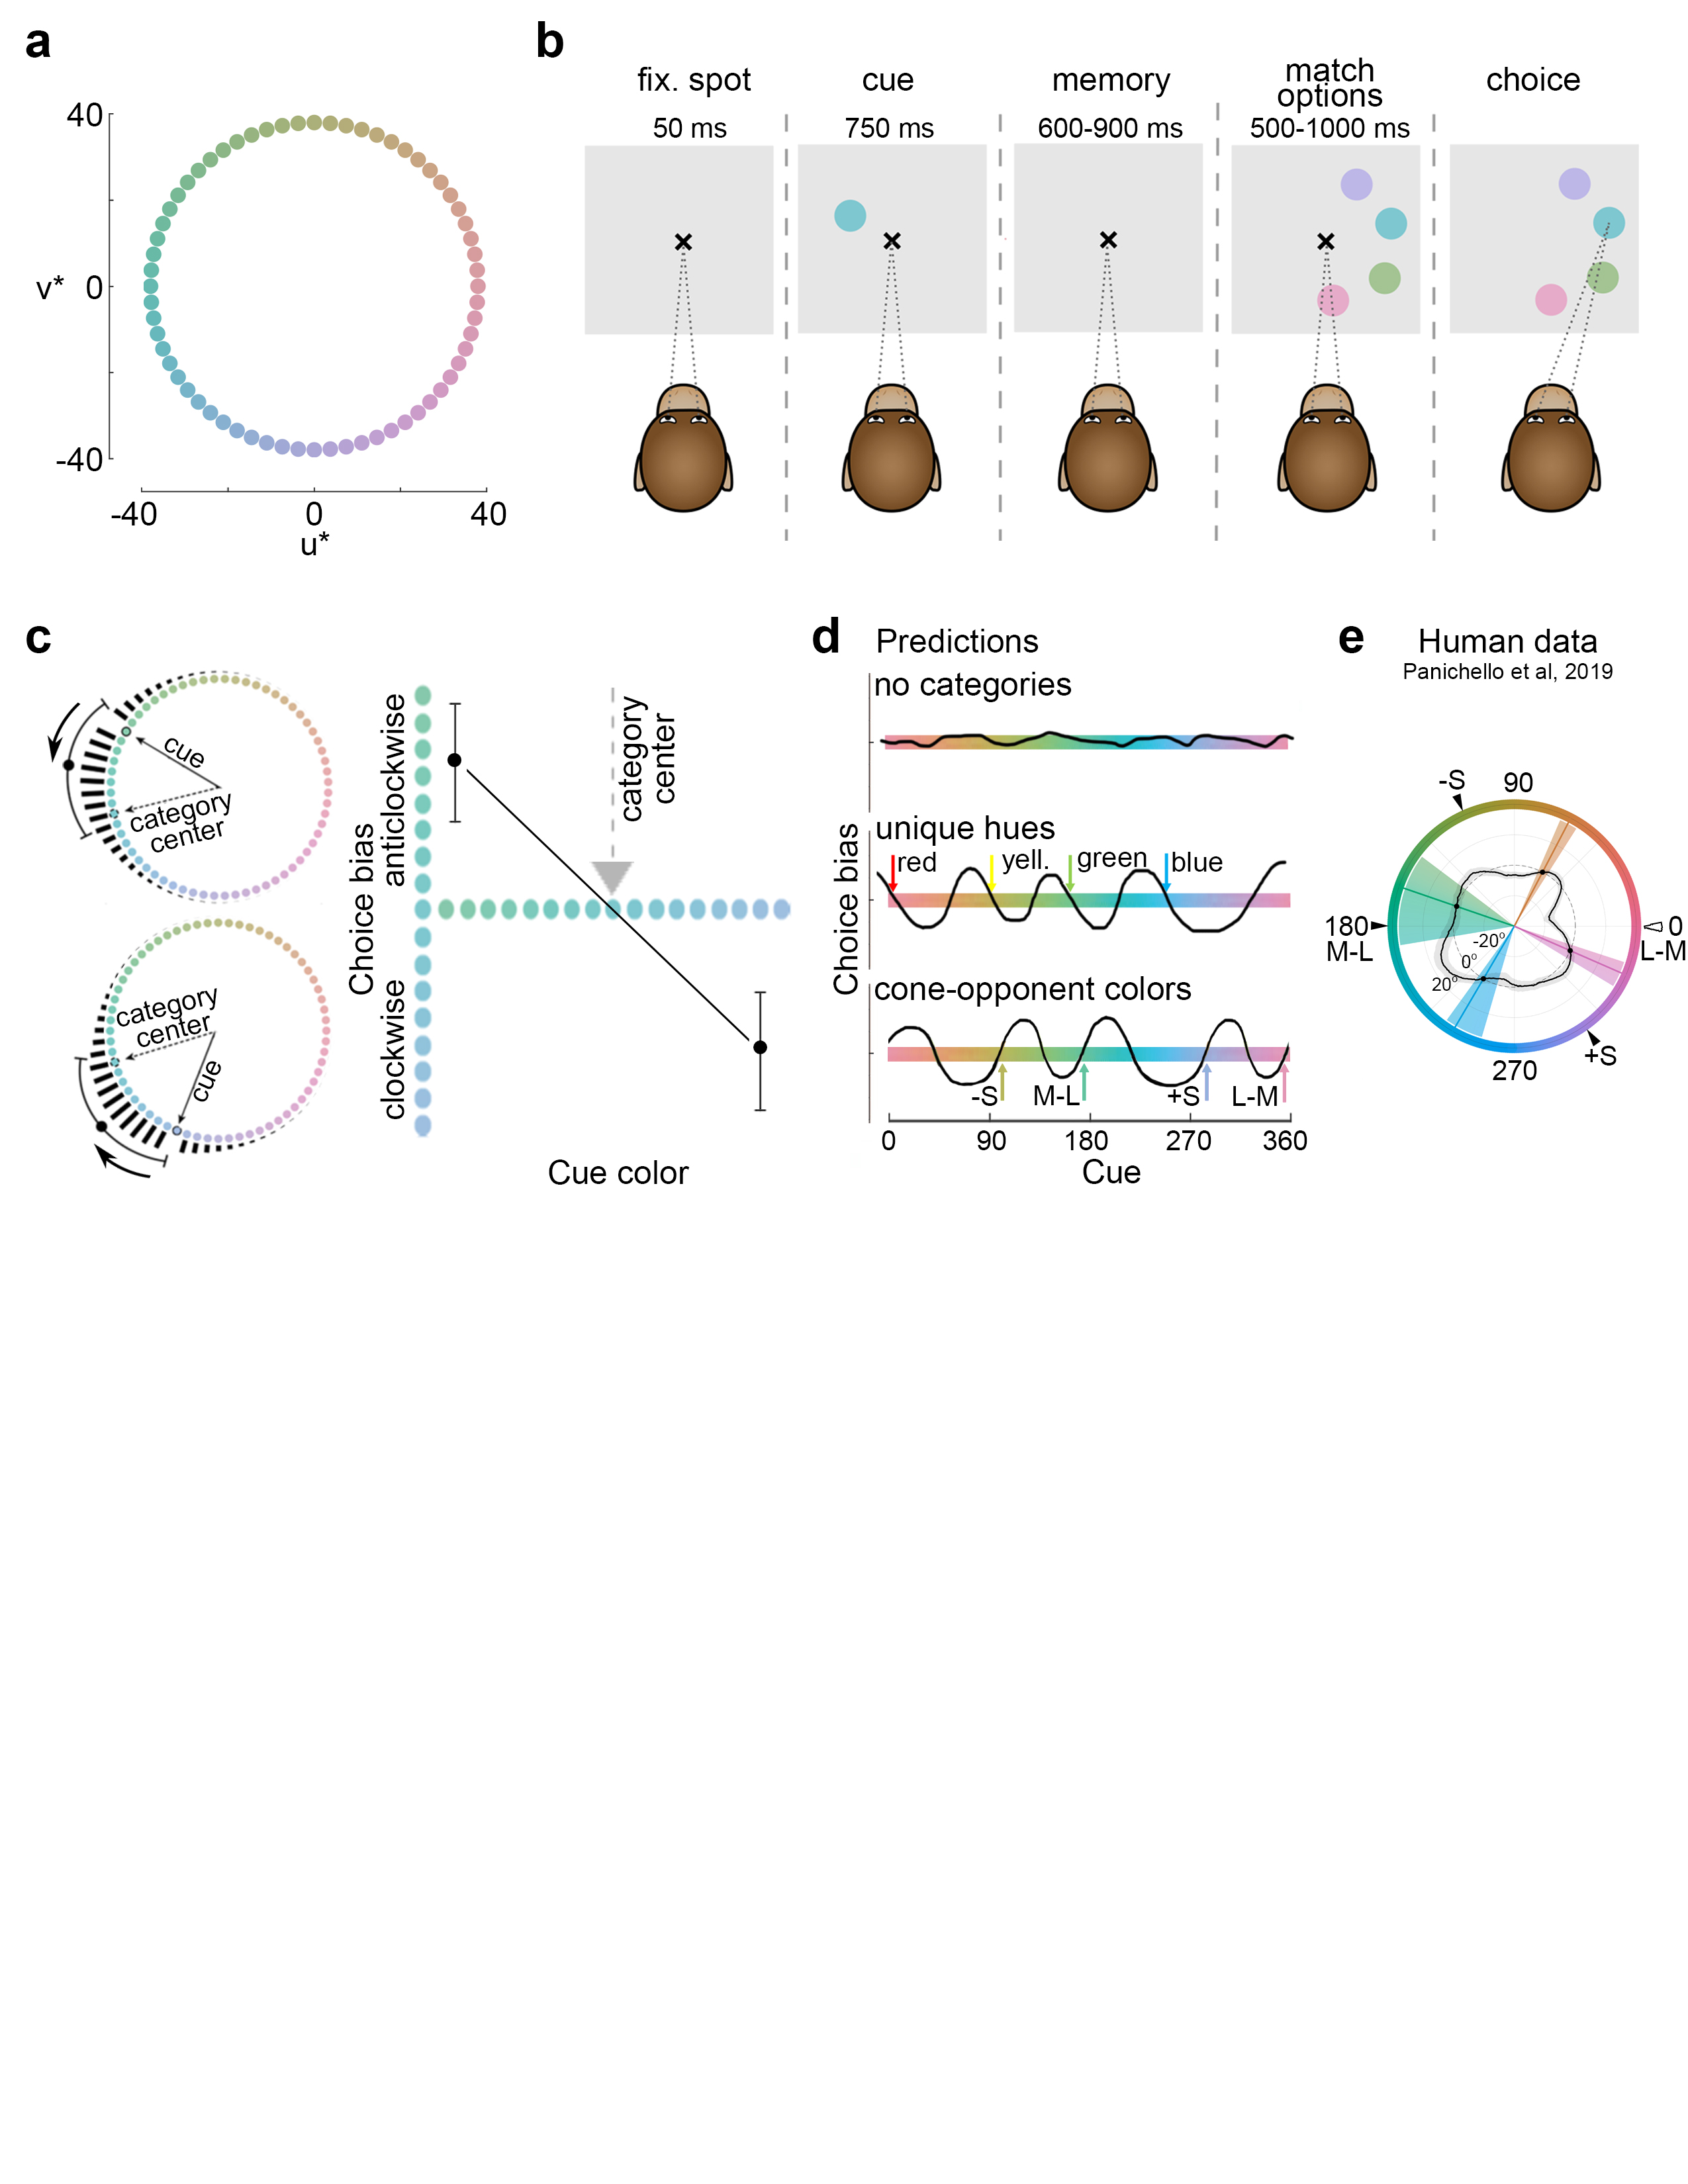
\includegraphics[width=\textwidth+4cm,trim={0 12.5cm 0 0},clip]{../Figures/flat/Fig1_ParadigmPredictions_7.jpg}
    \caption{\textbf{Non-verbal paradigm to recover color categories in non-human primates.}
    \textbf{a}, Sixty-four Colors defined in CIELUV color space. 
	\textbf{b}, Animals were trained to initiate a trial by fixating a small cross on a computer monitor and to maintain fixation throughout the trial until the fixation cross disappeared, which was their instruction to make a choice; trials in which the animals broke fixation were aborted. 
	A 3-degree diameter cue was presented within the central 2.5 – 6-degrees, followed by a variable memory delay (600-900ms) and the presentation of four choice options. 
	To mitigate impulsive choices, the choice options were shown for a variable amount of time (500-1000 ms) during which the animals needed to maintain fixation to avoid aborting the trial. After the fixation cross disappeared, the animals were free to make their selection. 
	\textbf{c}, Predicted distribution of choices for two cues if a color category exists at the specified location in the color space (dashed arrow). 
	The average of the distribution of choices will be shifted counterclockwise from the cue if the cue is displaced clockwise to the category center (top) and shifted clockwise from the cue if the cue is displaced counterclockwise to the category center (bottom). This pattern of results would be captured as the zero-crossing of the negative slope in a plot of the choice bias versus cue color (right). 
	\textbf{d}, Predicted pattern of results for three hypotheses: no categories (top); categories defined by attractors to the four common basic color categories (middle); and categories defined by repellors to the cone-opponent retinal encoding mechanisms (bottom). 
	\textbf{e}, Data obtained in prior work on a related task in human subjects showing evidence of four color categories (see SI Figure 2 for three other data sets in human subjects, showing a similar pattern of results). The negative slopes demarking category centers are recovered by tracing the line in a counterclockwise direction, at points where the trace crosses the dashed circle marking zero choice bias. For reference, arrowheads show the colors that would maximally activate the retinal cone-opponent encoding mechanisms (L-M, M-L, +S, -S; where L, M, S are the three cone types).}
    \label{fig:ParadigmAnalysisPredictions}
    \end{fullwidth}
\end{figure}

Color categories are identified by color terms, of which the Basic Color Terms are considered prominent \citep{berlin_basic_1969}.
One hypothesis is that a subset of these terms express, such as red, green, blue, and yellow, express universal concepts \citep{heider_universals_1972,regier_focal_2005}
and are endowed by hard-wired neural mechanisms present at birth \citep{bornstein_categories_1976,lindsey_universality_2006}. 
This idea, put forth 150 years ago \citep{hering_zur_1875}, predicts common patterns in color naming across cultures \citep{baronchelli_modeling_2010,lindsey_hunter-gatherer_2015,abbott_focal_2016}
and finds some neurophysiological support in human infants \citep{clifford_electrophysiological_2009,yang_cortical_2016}. 
Behavioral work in infants also provides evidence for a biological origin of color categories \citep{franklin_new_2004,ozturk_language_2013} and suggests that color categories may build on an innate scaffolding defined by retinal cone-opponent mechanisms \citep{skelton_biological_2017}.
The infants in all these experiments were at least several months old, by which stage they would have had substantial cultural exposure, so the evidence that they express color categories cannot be conclusively ascribed to an innate origin. Another hypothesis is that color categories emerge in development, instructed by language and culture starting at birth \citep{davidoff_colour_1999,roberson_color_2005}, possibly involving an interplay of innate and developmental factors \citep{webster_variations_2002,kay_language_2006,franklin_lateralization_2008,regier_language_2009,paramei_online_2018}---such an influence of cultural factors would explain the variability in color naming patterns across languages \citep{davidoff_colour_1999,webster_variations_2002,roberson_color_2005,kay_language_2006,gibson_color_2017, paramei_online_2018}. Current consensus is that at least some aspect of color category behavior is acquired through experience. But the extent to which color categories are innate remains unresolved \citep{davidoff_nature_2009,RN18696,RN18699}.

An alternative approach to studying the origin of color categories could be provided by behavioral experiments in trichromatic non-human primates \citep{RN18699,siuda-krzywicka_biological_2019}. 
The few studies on this topic have come to different conclusions: one found color categories in macaque monkeys consistent with categories in human adults \citep{sandell_color_1979}, implying that color categories do not depend on language and may be innate.
This study inadvertently made comparisons substantially easier for cross-category than within-category trials, undermining its conclusion \citep{davidoff_cross-species_2010}. 
A later study tested for the existence of color categories across a limited range of colors and found a blue-green boundary in humans but not baboons \citep{fagot_cross-species_2006,RN18699}. The lack of color categories in the baboons might reflect the limited survey of color space or the choice of colors (blues and greens are categorized with high variability in all languages, including English \citep{gibson_color_2017}). A third study, designed to investigate visual working memory, had two animals match color samples to a continuous ring of colors; it was inconclusive about consensus color categories in monkeys because the two animals showed a different pattern of results \citep{panichello_error-correcting_2019}.

\paragraph{Measuring color categories in macaque monkeys}

Addressing the question of color categories in monkeys requires overcoming several challenges. First, how can color categories be measured without teaching the animals the categories or reinforcing idiosyncratic biases \citep{essock_color_1977,matsuno_color_2004}? Second, how should the color stimuli be specified \citep{siuda-krzywicka_biological_2019}? For example, specifying the colors as wavelengths \citep{sandell_color_1979} is not appropriate \citep{davidoff_cross-species_2010}. 
Third, how can data across the full circle of hues be obtained so as to avoid missing categories \citep{fagot_cross-species_2006}? A match-to-sample paradigm, using colors defined in a perceptually uniform color space \citep{stockman_colorimetry_2010} (Figure 1a), provides a potential solution to these challenges, because, as demonstrated for human subjects , color categories introduce biases in the distribution of matches \citep{bae_why_2015}. So color categories could be inferred from any observed biases without resorting to language. 

In the standard paradigm, the subject is asked to match the color of a cue to a continuous ring of colors \citep{wilken_detection_2004,zhang_discrete_2008,bae_why_2015,panichello_error-correcting_2019,schurgin_psychophysical_2020}, which works in human participants who can follow instructions but introduces complications in monkeys because it is not clear how to reward the animals. Rewarding them for picking a color in the vicinity of the color of the cue could reinforce idiosyncratic biases\citep{panichello_error-correcting_2019}; moreover, the response metric (an eye movement or pointed finger) could confound the perceptual decision with motor noise. So we adapted the paradigm as an alternative-forced-choice task in which a direct match to the cue was available in every trial and the monkeys were only rewarded for making the direct match (Figure 1b). The precision of the eye tracker (\textasciitilde0.3 degrees of visual angle) was considerably finer than the size of the choice options (3 degree diameter). One consequence of the adapted paradigm is that it requires a large number of trials to sample category performance across the space of colors. Four animals performed the task, completing a total of 209456 trials over 232 sessions (SI Figure 1).

If a monkey has a color category, the category center will be an attractor in the color space. An attractor would be captured by a zero-crossing of negative slope in a plot of choice bias (Figure 1c). Repellors, meanwhile, would be captured by zero-crossings of positive slope. The approach is data-driven, so it will recover whatever categories exist; nonetheless, before collecting the data we considered three possibilities. First, that the monkeys would show no color categories, predicted by the work sampling a limited range of colors in baboons \citep{davidoff_cross-species_2010} (Figure 1d, top). Second, that the monkeys would show four color categories, predicted by attractor points defined by basic color terms (Figure 1d, middle). Third, that the monkeys would show four color categories, but predicted by data in human infants corresponding to repellor points defined by cone-opponent mechanisms not basic color terms \citep{skelton_biological_2017} (Figure 1d, bottom). For reference, Figure 1e shows the results in human adults \citep{panichello_error-correcting_2019}. These results have been replicated by several groups, across multiple versions of the task including the discrete-matching version used presently (SI Figure 2). Note that the data do not perfectly line up with color categories predicted by the four most common basic color terms (red, yellow, green, blue). Instead they correspond to pink, orange, green, blue. The discrepancy may arise because of limitations imposed by ensuring equal saturation and luminance among the colors (the resulting set of stimuli have neither a good red nor a good yellow) (see \citep{bae_why_2015}). 


%\section{Results}
%
\paragraph{Monkeys exhibit biases} %hallmarks of color category behavior

The animals examined show a hallmark of color categorization behavior: memory biases towards a set of particular points in a perceptually uniform colorspace.
In \autoref{fig:BiasCurves} it can be seen that the biases deviate substantially and systematically from zero, with the attractor points being found where the bias line crosses the zero line from positive to negative (going counter-clockwise). These points are highlighted with colored lines, with the filled areas around these lines showing the confidence intervals on these crossing points. Repeller points found where the line crosses the zero line from negative to positive.

\begin{figure}
\includesvg[width=\linewidth]{../../../Analyses/combined/combined_categorybias2_230214.svg}
\caption{\textbf{Bias as a function of hue, for data collapsed over 4 animals.} 
}
\label{fig:BiasCurves}
\end{figure}

\paragraph{Shared color categories across monkeys}

We see that all tested monkeys share two common attractor points, which we interpret as evidence of two shared color categories: a warm/orange-ish category (between 0$^\circ$ and 45$^\circ$), and a cool/blue-ish category (between 180$^\circ$ and 225$^\circ$).

\paragraph{Individual differences between monkeys}

In one animal we see evidence of additional categories: strong evidence for a greenish category and weak evidence for a purple category (the ``strength" of a category can be gleaned from looking at the local gradient at the zero-crossing point)

% Results table?

%\begin{figure}
%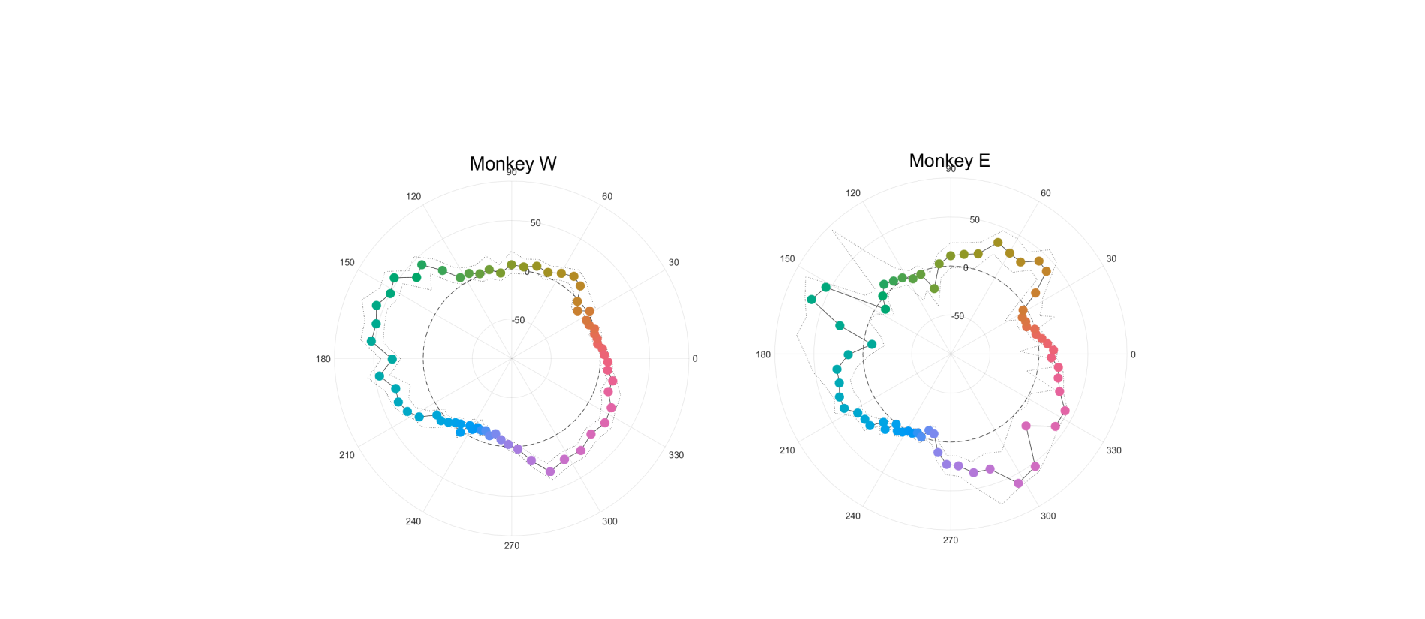
\includegraphics[width=\textwidth]{../../Figures/Old/panichellobias.pdf}
%\caption{Bias as a function of hue, for Panichello monkeys} 
%\end{figure}

\paragraph{Biases Compared to Humans}

Comparison to \cite{bae_why_2015}

Comparison to \cite{panichello_error-correcting_2019}

\paragraph{Cognitive Bias vs. Non-uniformity in Perceptual Space}

\begin{figure}
\includesvg[width=\linewidth]{../../../Analyses/combined/combined_TCC_230214.svg}
\caption{\textbf{Free Similarity model fit for combined data from all animals}
Similarity between stimulus $s_i$ and stimulus $s_j$, where one is the cue and one is the choice. This is a ``free'' similarity matrix - in that no particular relationship is pre-supposed between any of the stimuli (such as, for example: closer stimuli will be more similar). This figure can be compared to Figure 1D in \cite{schurgin_psychophysical_2020}, except there the rows are circularly shifted so that the the x-axis becomes the relative distance, rather than the absolute value of the stimulus. % should we just plot it the same way at this stage? It doesn't really make a difference here...
% supplementary figure with alternative plotting method?
%confidence intervals?!?!?! !!!!!!!!!!!!!!
} 
\label{fig:SimilarityMatrixCombined}
\end{figure}

\begin{figure}
    \centering
    \begin{subfigure}[b]{0.49\textwidth}
         \centering
         \caption{}
         \includesvg[width=\textwidth]{../../../Analyses/210609_124628_Buster/TCC_Buster_20230213.svg}
         \label{fig:SimilarityMatrixPollux}
    \end{subfigure}
    \hfill
    \begin{subfigure}[b]{0.49\textwidth}
         \centering
         \caption{}
         \includesvg[width=\textwidth]{../../../Analyses/210609_124628_Buster/TCC_Buster_20230213.svg}    
         \label{fig:SimilarityMatrixCastor}
    \end{subfigure}
    
    \begin{subfigure}[b]{0.49\textwidth}
         \centering
         \caption{}
         \includesvg[width=\textwidth]{../../../Analyses/210609_124628_Buster/TCC_Buster_20230213.svg}    
         \label{fig:SimilarityMatrixBuster}
     \end{subfigure}
     \hfill
     \begin{subfigure}[b]{0.49\textwidth}
         \centering
         \caption{}
         \includesvg[width=\textwidth]{../../../Analyses/220823_081207_Morty/TCC_Morty_20230213.svg}    
         \label{fig:SimilarityMatrixMorty}
     \end{subfigure}
        \caption{\textbf{Free Similarity model fits combined for individual animals} blabalbla}
        \label{fig:SimilarityMatrixIndividual}
\end{figure}


\paragraph{Longitudinal analysis}

Segmenting our data into subgroups of 5000 datapoints allowed us to both look at whether the determined categories varied over time, and also allowed us to perform a power analysis. From the monkeys studied it was clear that during our data collection period the categories remained static (within our measurement uncertainty), and also that the categories we saw are reliable enough to be seen with substantially less data. See Figures XXX % \autoref{}

%\clearpage
%\section{Discussion}
%
\paragraph{Locations of category centers.}

In the absence of language, we can infer that the shared categories we observe arise either due to innate biological factors, environmental factors such as the distribution of colors in the terrestrial environment, or a combination of the two.
The categories that we identify align well with the daylight locus (the line between the blue of the daytime sky, and the yellow of the sun, which itself closely follows the planckian locus), and also the warm/cool object/background distinction previously identified \citep{rosenthal_color_2018}. It is plausible that what we observe is the presence of two fundamental categories - `likely to be object of interest' and `likely to \emph{not} be object of interest'. 

\paragraph{Limitations of colorspace.}

For these experiments we used a nominally perceptually-uniform colorspace: CIELUV. This space has been derived psychophysically, with the goal of minimizing differences in perceptual non-uniformity across the space, for color differences of small magnitudes (the apparent color difference between two points in one part of the space should be equal to the apparent color difference between two points in another part of the space, given that the cartesian distance between the two points in each case be the same).

However, non-uniformities within the space are known to exist (ref?), and uniformity for small color differences does not necessarily assure uniformity for larger color differences (ref? Teunissen?). Likewise, uniformity for the conditions under which the psychometric measurements from which the space was determined (considering: spatial, temporal, spectral etc.) does not necessarily assure uniformity across all possible viewing conditions (ref).

With this in mind, it is reasonable to consider what the effect of residual non-uniformity might be on the results of our experiment. As discussed by \cite{panichello_error-correcting_2019} (their Figure S5) non-uniformities in colorspace could also potentially lead to systematic biases on tasks such as ours. The logic goes as follows: our points are uniformly distributed in our chosen space (\autoref{fig:StimuliAndParadigm}A), but if this space is actually non-uniform compared to the colorspace implicitly being used by an observer, then these same points will be \emph{non}-uniformly distributed in a hypothetical `perfect colorspace'. It follows that for each cue color, surrounding distractor points might actually be closer or further away than anticipated. If the nearest neighbors on one side of the cue are actually chromatically closer than the neighbors on the other side, one would expect these to be chosen at a higher frequency than the others, creating a systematic bias.

Unfortunately, these biases act in a similar fashion and are difficult to separate from one another. One potential way to distinguish one type of bias from another is to consider the theoretical relationship between bias and variance: if biases arise due to non-uniformities in colorspace, we would expect the attractor points to also have the \emph{highest} variance in responses. This is because in the hypothetical `perfect space' these points are actually tightly clustered, and so in the presence of noise we can assume that they will be frequently picked over one another. Conversely, at attractor points in spaces where the bias results from categoricality, theory would predict that we would see the \emph{lowest} levels of variance - if these points are conceptualized as `magnets' or `valleys' then we would expect cumulative noise to preferentially return to the attractor point, reducing the variance in responses.

In our data, we see...

[Compare to Bae/Panichello]

\begin{figure}
%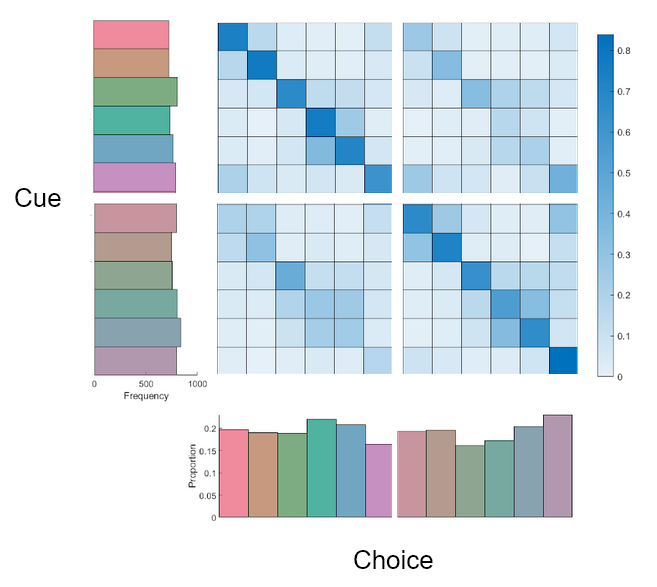
\includegraphics[width=\textwidth]{../../Figures/saturationBias.png}
\includesvg[inkscapelatex=false, height=\textwidth]{../../Figures/working/Poster_components/SD_Pollux copy.svg}
\caption{\textbf{}}
\label{fig:SamplingBias}
\end{figure}
\paragraph{Saturation bias.}

Non-uniformities in CILUV may also plausibly result in our nominally iso-saturated colors actually being variably saturated. This would be a concern, as it would be a reasonable prediction that higher saturation colors would be more salient, and thus more likely to be selected as responses. In a control experiment we see no (or very little) bias towards higher saturation colors. In \autoref{fig:saturationBias} it can be seen that there are a reasonable number of errors where an animal picks a higher saturation version of the same hue (lower left quadrant), but it is also seen that the number of errors of the inverse type (upper right quadrant) are roughly equal in number.


\begin{figure}
%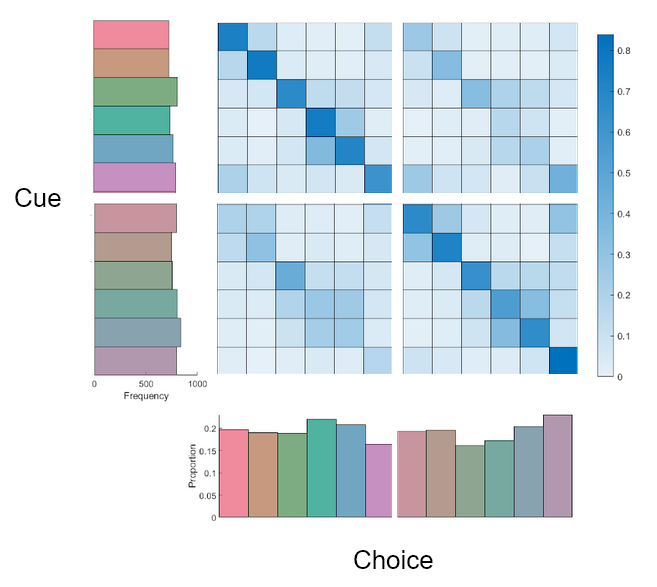
\includegraphics[width=\textwidth]{../../Figures/saturationBias.png}
\includesvg[inkscapelatex=false, width=\textwidth]{../../Figures/working/Poster_components/Saturation copy.svg}
\caption{\textbf{Saturation Bias.}
Heatmap of cues and corresponding choices. Selections along the negative diagonal correspond to correct choices. Choices along the negative diagonal in the bottom left and top right quadrants show trials on which an incorrect choice was made in such a way that the hue was correct but the higher or lower saturation versions of the cue were chosen (respectively). Note: the main diagonal is expected to be filled in at a greater extent regardless of performance level, since the correct choice is shown on every trial, whereas only a subset of the incorrect choices are shown.}
\label{fig:saturationBias}
\end{figure}



\paragraph{Comparison with humans} % /Panichello

%\section{Limitations}

%\section{Conclusion}

% \section{Acknowledgments}

Joshua Fuller-Deets adapted code from Shay Ohayon to create the experimental paradigm; Rosa Lafer-Sousa collected pilot data; Whitney Teagle and Shriya Awasthi assisted data collection. 
Funding was provided by the Intramural Research Program of the National Eye Institute. 
We are thankful to the animal care team lead by Denise Parker and Hayden Warnock and to the veterinary staff of the NEI for excellent animal care. 
We thank members of the Laboratory of Sensorimotor Research, attendees of the Colour Group of Great Britain’s January Vision Meeting (2022), the Vision Sciences Society (2022, 2023), the Society for Neuroscience (2023), and the Color Workshop sponsored by the University of Giessen (Summer 2023) for helpful feedback. 
We thank Thorsten Hansen for consultation on color conversions, Ramon Bartolo for mathematical assistance, and Karl Gegenfurtner for the initial prompt to think about testing for color categories in macaques.

\newpage
\section{Author contributions}

% table? e.g. https://twitter.com/AnneEUrai/status/1361356189284581387

% 'CRediT' (https://casrai.org/credit/)

Conceptualization: BRC, DJG\newline
Data curation: DJG\newline
Formal Analysis: DJG, HMS, ALYC\newline
Funding acquisition: BRC\newline
Investigation: all authors\newline
Methodology: all authors\newline
Project administration: BRC\newline
Resources: BRC\newline
Software: DJG, HMS, ALYC\newline
Supervision: BRC\newline
Validation: DJG\newline
Visualization: all authors\newline
Writing – original draft: BRC, DJG\newline
Writing – review \& editing: BRC, DJG\newline


\clearpage
\printbibliography[title=Main Text References]
\end{refsection}

% DON'T EDIT. If "endfloat" option is enabled all floats appear before appendices
\if@endfloat\clearpage\processdelayedfloats\clearpage\fi 

\begin{refsection}
\newpage
\section{Methods}
\subsection{Subjects}
Data were collected in four adult male rhesus macaques (Macaca mulatta)(“PO, CA, BU, and MO”) weighing 8–10 kg. 
All experimental procedures were approved by the Animal Care and Use Committee of the National Eye Institute and complied with the regulations of the National Institutes of Health. 
Plastic headposts were mounted with sterile surgical procedures, using procedures described in detail elsewhere \citep{lafer-sousa_parallel_2013}. 
The animals were acclimatized with positive reinforcement to sit in a custom-made chair positioned with the eyes 57 cm in front of a computer monitor and to perform visual tasks as described below. 
\subsection{Behavioral task}
\paragraph{Stimuli.} 
Stimuli were discs presented on a XXX screen.
The color of stimuli varied only in hue, and were sampled from 64 equally spaced points on a circle in CIELUV space (\autoref*{fig:paradigm}, \autoref*{fig:suppTest}), with a white point of XXX (xy), a radius of 37, and a luminance of XXX (L* = 76.0693). These values were chosen to maximize gamut while maintaining a fixed saturation and luminance. The background was XXX.
% g_astrctAllParadigms{1, 1}.m_strctConversionMatrices.RGBToXYZ
% Kofiko\Paradigms\CommonFunctions\luv2rgb.m
CIELUV was used, in contrast to previous work which has used CIELAB, because CIELUV has the benefit of an associated chromaticity diagram. 
We also noted that nominally equi-saturated stimuli defined in CIELAB tended to have significant variation in apparent saturation, whereas the same in CIELUV were much closer to visually equi-saturated. 
Luminance noise was added by XXX to the extent of YYY.
% Kofiko\Paradigms\CommonFunctions\fnGenerateNoisePattern.m
% Kofiko\Paradigms\TouchForceChoiceColorCategories\fnInitializeCueTrainingTextures.m (line 144)
% Kofiko\Paradigms\TouchForceChoiceColorCategories\fnParadigmTouchForceChoiceColorCategories\Callbacks.m (line 613)


The experiment was controlled by multiple computers running `Kofiko' (a MATLAB/Psychtoolbox (ref) based software for working with monkeys).

\paragraph{4-Alternative Forced Choice (4-AFC): Non-human primates.} Non-human primates were trained on a color-matching task. Trials begin with fixation (50 ms) on a white cross in the center of the screen. A cue stimulus (colored disc) is shown to one side of the fixation cross (750 ms). The position of the cue is invariant throughout a daily session. Following cue presentation, the monkey must maintain fixation (600-900 ms) before the choice stimuli appear on the screen alongside the fixation cross (500-1000 ms). The choices are positioned at constant eccentricity and with equal spacing in the hemifield opposite the cue stimulus, with the exact positions of the stimuli varying randomly trial-to-trial. One choice is always a direct match to the cue, and the other three are randomly sampled. Upon offset of the fixation cross, the animal makes a selection by saccade, and is rewarded for selecting the choice that is identical to the cue. Animals were head-fixed at a distance of XXX from the screen. Stimuli had a radius of XXX degrees of visual angle, at an eccentricity of XXX/degrees from a central fixation.
% Diameter of cue/choice discs: 2.89 degrees (100 px)
% Distance between cue and choice: 5.79 degrees (200 px - g_astrctAllParadigms{1, 1}.m_strctCurrentTrial.m_strctChoiceVars.choiceRhos)
% Diameter of “fixation window”: 1.58 degrees (50 px)
% Audrey going to re-check

\paragraph{4-Alternative Forced Choice: Human participants.} Human participants were recruited via Amazon Mechanical Turk to perform an analogous version of the non-human primate 4-AFC task. Participants click on an initial fixation cross to request a trial, after which a cue is shown to one side of the fixation cross (750 ms). After cue offset, a fixation cross is shown and the cursor is hidden to de-incentivize mouse movement (1500 ms). Four choices are then shown, and participants make their selection by clicking. 

\paragraph{Pseudo-continuous color matching task: Human participants.} All 64 stimuli were displayed in a ring at XXX eccentricity. 

\begin{figure}
\includesvg[inkscapelatex=false, width=\textwidth]{../../Figures/F1_StimuliAndParadigm_1.svg}
\caption{\textbf{4-Alternative Forced Choice (4-AFC) Paradigm.}
\emph{A.} Cue and choice colors in the u*v* plane of CIELUV. Colors were defined to be equi-luminant and equi-saturated in CIELUV.
\emph{B.} Cue and choice colors in DKL colorspace.
\emph{C.} The timing and visual organisation of the delayed match-to-sample task that the animals performed.
} 
\label{fig:paradigm}
\end{figure}

\paragraph{Color-naming task} [DANNY - get info from Sihan?]



% Distance between cue and choice: 5.79 degrees (200 px - g_astrctAllParadigms{1, 1}.m_strctCurrentTrial.m_strctChoiceVars.choiceRhos)


\subsection{Data Analysis}

\paragraph{Mixture Modeling}\label{para:MixtureModeling}

To assess the bias in responses for each cue, we computed the distribution of responses on trials where the monkey made an incorrect choice.
For each completed trial, we calculated the error as the angular difference between the correct option and the chosen option.  
For each cue, we computed the number of times the monkey selected each incorrect choice, normalized by the number of times each choice color was available as a choice option for all completed trials of the given cue (though this was approximately uniformly distributed).
We then fit a Gaussian with a variable floor (\autoref{eq:GaussianEquation}) to the error distribution for each cue, using the MATLAB \lstinline{fit} function with the equation defined as \lstinline{a*exp(-(((x-b)^2)/(2*c^2)))+d}. 

% demo annotated-equation code from here: https://mirrors.concertpass.com/tex-archive/macros/latex/contrib/annotate-equations/annotate-equations.pdf

%\newpage %Sometimes the annotations don't show up, the hacky solution is to force them onto a new page

\vspace{2em} 
\begin{equation} \label{eq:GaussianEquation}
    \eqnmarkbox[purple]{p1}{a}
    \cdot
    \exp
    \frac{-(x-
    \eqnmarkbox[violet]{mu}{\mu}
    )^2}{2 
    \eqnmarkbox[blue]{sigma}{\sigma}^2}
    +
    \eqnmarkbox[gray]{d}{d}        
\end{equation}

\annotate[yshift=1em]{above,left}{p1}{height of the curve's peak}
\annotate[yshift=1em]{above}{mu}{position of the center of the peak}
\annotate[yshift=-0.75em]{below,left}{sigma}{standard deviation}
\annotate[yshift=-1em]{below}{d}{floor}
\vspace{2em} 

This fit was weighted by the number of times each choice color was an option for the given cue across all completed trials (though as before, this was approximately uniformly distributed). 
Bias was taken as the difference between the cue and the peak of the corresponding Gaussian, for each cue color ($b$ in \autoref{eq:GaussianEquation}). 
%These values were then smoothed (with a circular moving average filter of 5 cues) since our primary interest was in the broader structure of the bias distribution, and this is shown as the black lines in \autoref{fig:BiasCurves}.
These values, for each stimulus, are plotted as the black lines in \autoref{fig:BiasCurves}.
Where this line falls closer to the center of the figure than the 0$^{\circ}$ line, there is negative bias (which in this representation is counter-clockwise), and vice versa for values above the 0$^{\circ}$ line.
%Attractor points (thought to indicate color category centers) occur where the bias curve crosses the zero line from positive to negative (going counter-clockwise).
%At these points, there is zero bias, and hues on either side provoke choices that are biased inwards towards this point.
%Correspondingly, repeller points occur where the bias curve crosses the zero line from \emph{negative to positive} (again, going counter-clockwise).
%At these points there is also zero bias, but hues either side of this point are biased \emph{away} from this point.
Confidence intervals were extracted from 

%\subparagraph{Confidence intervals}
%To find the 95\% confidence intervals for the locations of the category centers, we performed 1000 bootstraps on all completed trials. For each bootstrapped sample, we found the bias values for each cue color, smoothed the bias curve, and found the category center locations for each bootstrapped dataset. To find the category center locations for the full data set and their confidence interval, we found the category boundaries and segmented all bootstrapped category centers that fell between two consecutive category boundaries. For each of these segments, we found the circular mean and circular standard deviation of all category crossings that fell within these boundaries. 
%\begin{figure}
%\includesvg[inkscapelatex=false, width=\textwidth]{../../Figures/F2_DataAnalysis_v2.svg}
%\caption{\textbf{Task performance.}
%Performance as a function of trial difficulty, quantified as the closeness of the chromatically closest incorrect choice.
%\emph{A.} For one animal, with five example choice sets below for trials where the cue was cue \#28 (correct choice highlighted by dashed line here, not visible to animal).
%\emph{B.} For all animals.
%} 
%\label{fig:TaskPerformance}
%\end{figure}

\paragraph{Target Confusability Competition (TCC)}\label{para:TCC}
One disadvantage of the mixture model for our analysis is that we can only use it to analyze the subset of trials where the animal made an incorrect response\footnote{
This is for messy and annoying reasons. 
Firstly, since in our paradigm the choices consist of ``the correct choice'' plus three ``distractors'' (see \nameref{para:4AFC}), the correct choices are greatly over-represented. 
Imagine: by guessing at random, the correct choice would be picked far more frequently than any of the other stimuli, since it is presented on \emph{every trial}, whereas the other stimuli are only presented as distractors with a probability of $\frac{1}{63} + \frac{1}{62} + \frac{1}{62}$. 
This could be normalized out, as we do for the other values, but then a more insidious issue becomes apparent: 
For ``high-error'' choices, the odds of there being a similar choice to that one is less than the odds of there being a similar choice to the ``0-error'' choice, and thus the probability of selecting the correct answer, when normalised, is lower than one would expect. 
%Or to flip the logic: there are slightly higher odds of there being a close distractor to the 0-error stimulus than there is to a high-error stimulus.
You can think of it as: for the high-error choice, there are \emph{2 chances} to pick another choice option that is close to the high-error choice (since one choice is going to be the distant-by-definition 0-error choice), whereas for the 0-error choice there are \emph{3 chances}.
%2 comes from: 1 already used to be the 0-error choice, which by definition is not close to the high-error choice. And 1 is the high error choice itself, so you have 2 left to place.
An additional note for clarity: this is an issue for us because of the sampling required for the AFC paradigm, and is not an issue of concern for those who use a response mechanism where all possible responses are simultaneously presented.
}.
In order to use the full dataset (both incorrect and correct trials), we developed a generative model, based on the \emph{Target Confusability Competition (TCC)} model of \cite{schurgin_psychophysical_2020}.
The key elements of the TCC model are a similarity function, which determines the similarity between stimulus $s_i$ and stimulus $s_j$ and a value of $d'$, which can be thought of as describing the amount of noise acting on the system. 
Taken together, these two elements can be used to predict the probability that a choice of colour $s_j$ will be picked, from the set of $[s_{j1} ... s_{jn}]$, on a trial where the cue is $s_i$.
Our implementation of the model differs in some key ways to that described in \cite{schurgin_psychophysical_2020}:
\begin{enumerate}
\item We do not assume that the underlying function is the same for each stimulus. 
\cite{schurgin_psychophysical_2020} collapse across stimuli for the majority of their analyses (though, see their Figures 1D and Extended Data Figure 5). 
Since we are most interested in the differences between the functions for the different stimuli, it does not make sense for us to collapse our data. 
We therefore deal with a ``similarity matrix'', whereas \cite{schurgin_psychophysical_2020} could refer to their collapsed version as a ``similarity function''.
\item We make no assumptions about the underlying function that determines similarity. \cite{schurgin_psychophysical_2020} use an exponential function with additional perceptual noise (see their Figure 1F), based on observations gained from collecting data on various simultaneous judgment tasks. We choose not to do this, because we expect that if biases are present, this would modify the shape of the function differently for each stimulus. We refer to fits made this way as ``free similarity matrix'' fits, since each elements of the matrix is ``free'' to float as it wishes, independently of those elements around it.
\item We fit our model on a single dataset, whereas \cite{schurgin_psychophysical_2020} derive their similarity functions and values for $d'$ from independent datasets. % why do they do this?
\item In fitting a ``free similarity matrix'' noise in the system can either be represented by the value of $d'$ or in modifying the ``contrast'' of the similarity matrix (the relationship between the highest values and the lowest values in the matrix), since we apply no constraints on the floor or peak of the function. 
We therefore assume a value of $d' = 1$ for free similarity matrix fits. %and only actively fit $d'% in (these other models)...
\item Since we use an AFC method, as opposed to a pseudo-continuous response space, we are able to take advantage of an alternative computational method for computing the probabilities of a particular choice being made.
We use the correction factors of \cite{mcgraw_common_1992} (their Table 3) to estimate the probability $P(X_1>max(X_2,X_3,X_4))$, where $X_{1:4}$ are samples from independent normal variables, with means representing the pairwise similarity values between $s_i$ and $s_j$, and variances determined by $d'$.
This decreases the runtime of our model by several orders of magnitude compared to the method used by \cite{schurgin_psychophysical_2020} (See the function \lstinline{modelPDF} in \lstinline{TCC_Code_InManuscriptOrder\Model\TCCUncorrelated.m} from \url{https://osf.io/j2h65/} for comparison).
\end{enumerate}

Using this model, we used parameter estimation techniques to construct a similarity matrix where each cell represented the similarity between stimulus $s_i$ and stimulus $s_j$. 
Such a similarity matrix is shown in \autoref{fig:SimilarityMatrixPollux} for a single animal (Monkey P).
This model, and this visualization method, allows us to assess not only the mean of the bias in the responses, but the shape of the response-bias-curve, which gives us an insight into the source of the bias.

\paragraph{Distinguishing between cognitive biases and biases arising from non-uniformity of stimulus space}

For these experiments, we used a nominally perceptually-uniform colorspace: CIELUV. 
This space has been derived psychophysically, with the goal of minimizing differences in perceptual non-uniformity across the space, for color differences of small magnitudes (the apparent color difference between two points in one part of the space should be equal to the apparent color difference between two points in another part of the space when that the cartesian distance between the two points in each case be the same).

However, non-uniformities within the space are known to exist (ref?), and uniformity for small color differences does not necessarily assure uniformity for larger color differences (ref? Teunissen?). % no color space is perfect etc
Likewise, uniformity for the conditions under which the psychometric measurements from which the space was determined (considering: spatial, temporal, spectral etc.) does not necessarily assure uniformity across all possible viewing conditions (ref).

With this in mind, it is reasonable to consider what the effect of residual non-uniformity might be on the results of our experiment. 
As discussed by \cite{panichello_error-correcting_2019} (their Figure S5) non-uniformities in colorspace could also potentially lead to systematic biases on tasks such as ours. % However, I think the they reach the opposite conclusion as we do...
The logic goes as follows: our points are uniformly distributed in our chosen space (\autoref{fig:StimuliAndParadigm}A), but if this space is actually non-uniform compared to the colorspace implicitly being used by an observer, then these same points will be \emph{non}-uniformly distributed in a hypothetical `perfect colorspace'. 
It follows that for each cue color, surrounding distractor points might actually be closer or further away than anticipated. 
If the nearest neighbors on one side of the cue are actually chromatically closer than the neighbors on the other side, one would expect these to be chosen at a higher frequency than the others, creating a systematic bias.
\cite{panichello_error-correcting_2019} lack a robust framework within which to test these ideas, and conclude that there would be no effect on their conclusions. We reach a contrary conclusion.

%Unfortunately, these biases act in a similar fashion and are difficult to separate from one another. One potential way to distinguish one type of bias from another is to consider the theoretical relationship between bias and variance: if biases arise due to non-uniformities in colorspace, we would expect the attractor points to also have the \emph{highest} variance in responses. This is because in the hypothetical `perfect space' these points are actually tightly clustered, and so in the presence of noise we can assume that they will be frequently picked over one another. Conversely, at attractor points in spaces where the bias results from categoricality, theory would predict that we would see the \emph{lowest} levels of variance - if these points are conceptualized as `magnets' or `valleys' then we would expect cumulative noise to preferentially return to the attractor point, reducing the variance in responses.

It is difficult to distinguish biases from different sources using the Mixture Modeling approach... %why?
% is it because TCC seperates out d' and simMatrix, whereas mixmod implicitly combines the two (by using a matrix that is directly "probability of choice"?)

This task becomes tractable in the TCC framework. (why?)
A reasonable definition of cognitive bias might be: an agent is more likely to pick choice $s_2$ as a match to cue $s_1$ than they are to select choice $s_1$ as a match to cue $s_1$, and that this behavior would not be reciprocal (they would not be more likely to pick choice $s_1$ as a match to cue $s_2$ than they are to select choice $s_2$ as a match to cue $s_2$).
By this definition, this type of bias would appear as spread or displacement away from the negative diagonal in the similarity matrix, that \emph{was not} symmetric across the negative diagonal (symmetry across the diagonal would represent reciprocity).
There are numerous ways that cognitive bias can be envisaged/implemented.
A cartoon example is shown in \autoref{fig:JustBias}.

Spread away from the negative diagonal which is mirrored across the diagonal represents non-uniformity of the stimulus space.
In areas where the behavioral space is oversampled, one would see spread away from the negative diagonal (adjacent colors are more similar than the average).
In areas that are undersampled, one would see a pinch into the negative diagonal (adjacent colors are less similar than the average).
A cartoon example is shown in \autoref{fig:JustColSpace}.

\begin{figure}
     \centering
     \begin{subfigure}[b]{0.45\textwidth}
         \centering
         \caption{}
         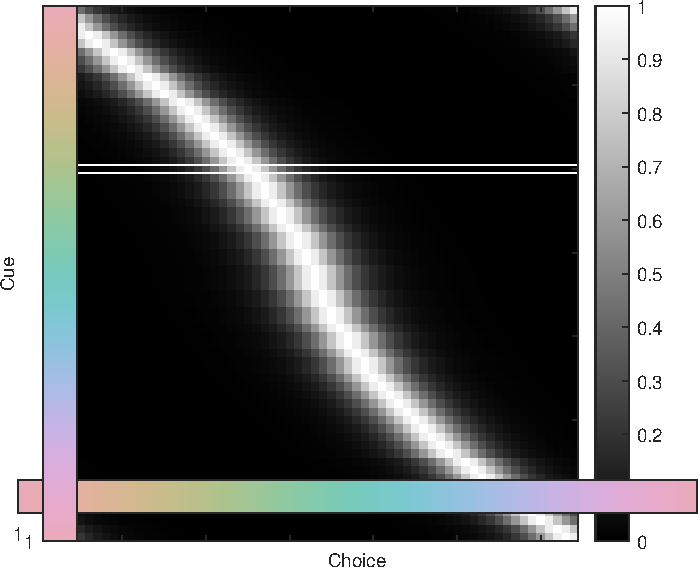
\includegraphics[width=\textwidth]{../../Figures/working/justBias.pdf}
         \label{fig:JustBias}
     \end{subfigure}
     \hfill
     \begin{subfigure}[b]{0.45\textwidth}
         \centering
         \caption{}
         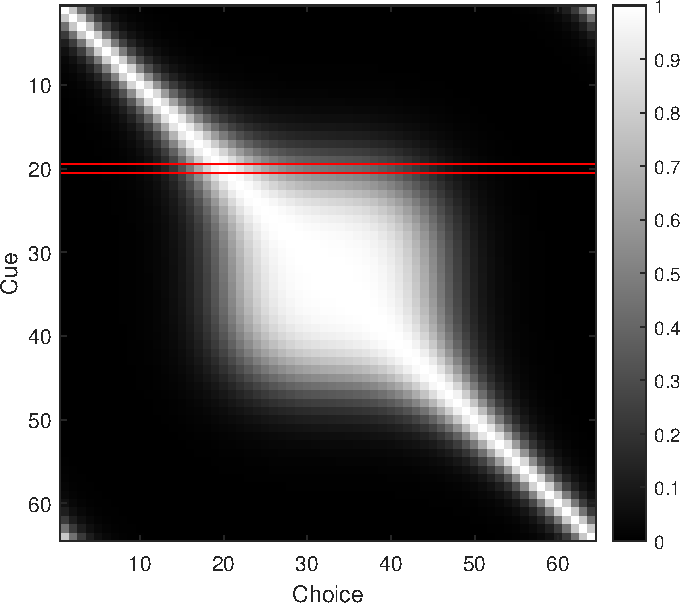
\includegraphics[width=\textwidth]{../../Figures/working/justColSpace.pdf}         
         \label{fig:JustColSpace}
     \end{subfigure}

          \begin{subfigure}[b]{0.45\textwidth}
         \centering
         \caption{}
         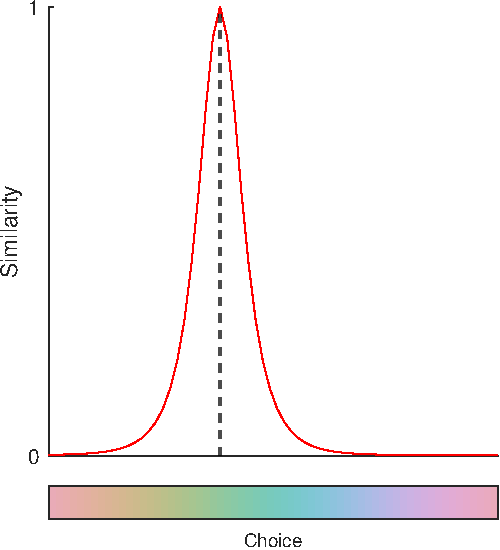
\includegraphics[width=\textwidth]{../../Figures/working/justBias_subset.pdf}
         \label{fig:JustBias_subset}
     \end{subfigure}
     \hfill
     \begin{subfigure}[b]{0.45\textwidth}
         \centering
         \caption{}
         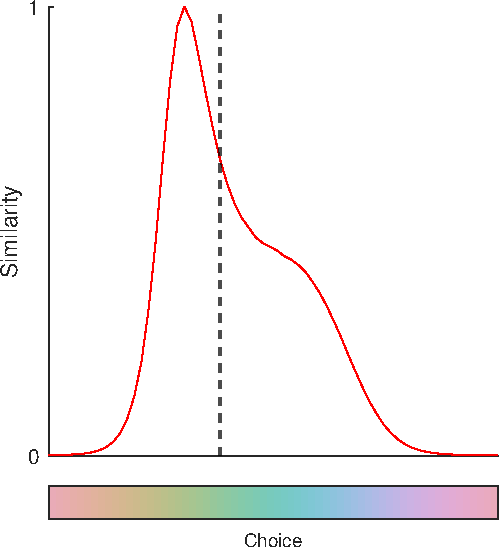
\includegraphics[width=\textwidth]{../../Figures/working/justColSpace_subset.pdf}
         \label{fig:JustColSpace_subset}
     \end{subfigure}
        \caption{\textbf{Distinguishing between different sources of bias using TCC models: cognitive bias vs. non-uniformity of stimulus space.} Similarity matrices representing different theoretically driven mechanisms can result in the same average bias value. A mixture model cannot distinguish between these different sources, whereas a TCC model readily can. \ref{fig:JustBias}: an example of how cognitive bias might appear - each row of the matrix is shifted leftwards or rightwards. \ref{fig:JustColSpace}: an example of how non-uniformity in stimulus space might appear - the similarity between each cue and its neighbors is increased or decreased, resulting in an expansion of the higher similarity region of the matrix symmetrically around the negative diagonal for colors which are more similar to their neighbors than average, and a contraction for colors that are less similar to their neighbors than average. \ref{fig:JustBias_subset}: The values representing the similarity function for cue 20 (the row highlighted in red in \ref{fig:JustBias}), with the circular median shown as a vertical dashed line. \ref{fig:JustColSpace_subset}: As in \ref{fig:JustBias_subset} but for \ref{fig:JustColSpace}. Note how the circular median of \emph{both} functions is 25}
        \label{fig:distinguishing}
\end{figure}

In this example, it is possible to see how responses could be biased even in the absence of cognitive bias - consider cue 20, for example. 
The similarity of cue 20 to all the possible choices is represented by the row of elements at location 20. Tracking left to right from the y-axis, see how there is only a small area of similarity to the left of the negative diagonal and a larger area of similarity to the right of the diagonal. 
Although the most similar choice is still 20, there is a longer tail of the similarity distribution to the right than to the left, and thus responses will be shifted to higher values on average. %illustrate? - by lines on graph, or by pulling out the individual? 

% this also affects standard deviation, which can be assessed in the mixture model...

To estimate how much of the bias could be attributed to non-uniformity of colorspace, we fit an alternative version of the TCC model. 
In this version, we use a single similarity function, defined by \autoref{eq:SimilarityFunction} (which is controlled by two parameters: $\lambda$ and $\sigma$, which together control the slope of the function and the extent of the flat-top of the function at zero)\footnote{These two parameters can be though of theoretically as the \emph{similarity function} (how similar is $x$ to $y$), and the \emph{perceptual function} (at what point do stimuli become indistinguishable from one-another). Unfortunately, in this parameterization of the function, the parameters are highly correlated, which makes recovery of these values via model fitting rather difficult. An alternative parameterization where the parameters were maximally uncorrelated would be preferable.} and instead allow the stimuli chromaticities to float.
This is akin to asking: what set of relationships between the stimuli in stimulus space can best explain the data we observe?
% do we fit the similarity function, or choose reasonable estimated values?

\renewcommand{\eqnhighlightheight}{\vphantom{\hat{H}}\mathstrut} %make the highlighted a standard height


\vspace{2em} 
\begin{equation} \label{eq:SimilarityFunction}
    \eqnmarkbox[purple]{explambda}{\exp(x\cdot\lambda)}
    \eqnmarkbox[cyan]{convolution}{\circledast}
    \eqnmarkbox[blue]{sigma}{\mathcal{N}(0,\sigma^2)}
\end{equation}

\annotate[yshift=1em]{above,left}{explambda}{scaled exponential}
\annotate{below,left}{convolution}{convolution}
\annotate[yshift=1em]{above}{sigma}{normal distribution with mean of 0 and standard deviation of $\sigma$}


% It would be possible to allow the stimuli to float in any number of dimensions, which might be useful for detecting luminance intrusion, or other unintended/unanticipated dimensions

% The rotation/offset in this space is arbitrary. It is all about relationships.

\vspace{2em} 

\paragraph{Reconstruction of colorspace}

...

%\begin{figure}
%\includesvg[inkscapelatex=false, width=\textwidth]{../../Figures/working/Poster_components/BiasCalculation copy.svg}
%\caption{Analysis and Hypotheses.} 
%\label{fig:BiasCalculation}
%\end{figure}


% Amazon Mechanical Turk Data

% Conversion between CIELAB and CIELUV

%\paragraph{Discrete vs. Continuous Response Space}
% MechTurk data vs. Bae/Panichello Humans
% Our monkeys vs. Panichello monkeys

%%%%%%%%%%%%%%%%%%%%%%%%%%%%%%%%%%%%%%%%%%%%%%%%%%%%%%%%%%%%
%%% SUPPLEMENTARY MATERIAL / APPENDICES
%%%%%%%%%%%%%%%%%%%%%%%%%%%%%%%%%%%%%%%%%%%%%%%%%%%%%%%%%%%%


% modified from: https://tex.stackexchange.com/a/611819/169285
\newcommand{\supplementarysection}{%
  \setcounter{figure}{0}% Reset figure counter
  \let\oldthefigure\thefigure% Capture figure numbering scheme
  \renewcommand{\thefigure}{S\oldthefigure}% 
}

\supplementarysection

\begin{figure}
    \centering
    \begin{fullwidth}
    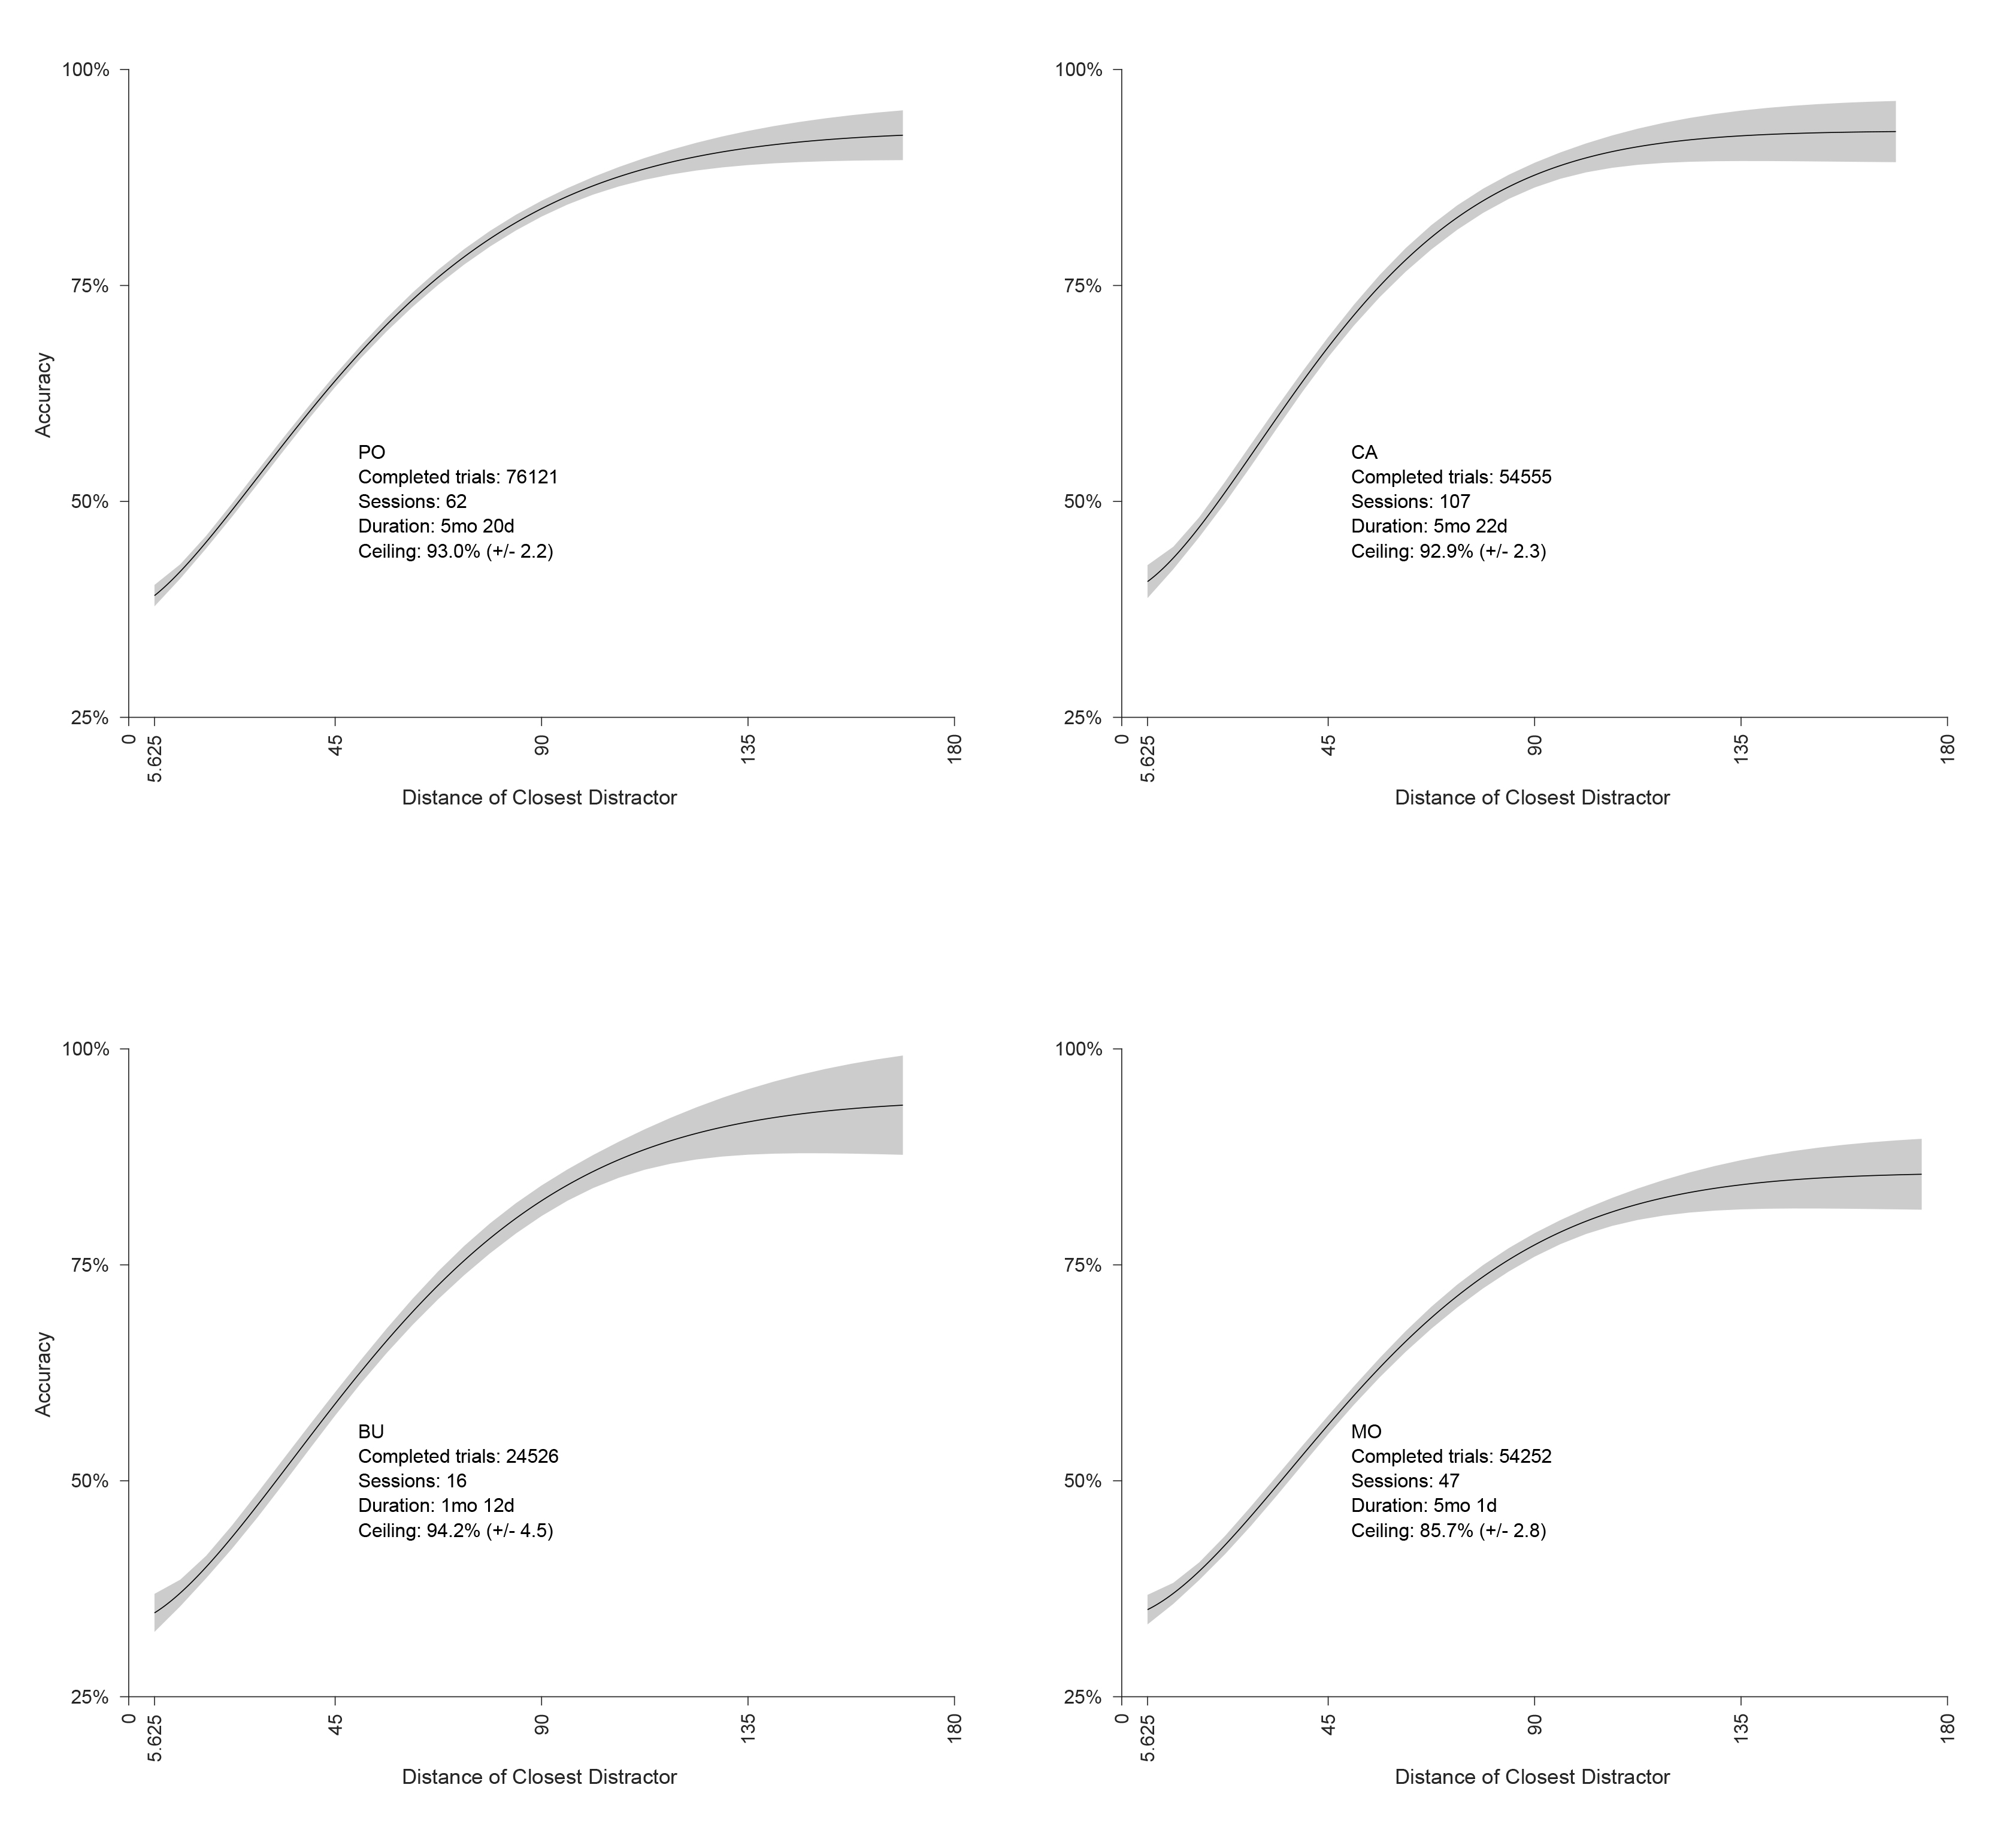
\includegraphics[width=\textwidth+4cm]{../Figures/flat/SI1_psychometric.jpg}
    \caption{\textbf{Psychometric functions for the four individual animals (PO, CA, BU, MO) on the color-matching task illustrated in Figure 1.}
    Completed trials for the four animals were: 76121; 54555; 24526; 54252.
    } 
    \label{fig:IndiDiff}
    \end{fullwidth}
\end{figure}

\begin{figure}
    \centering
    \begin{fullwidth}
    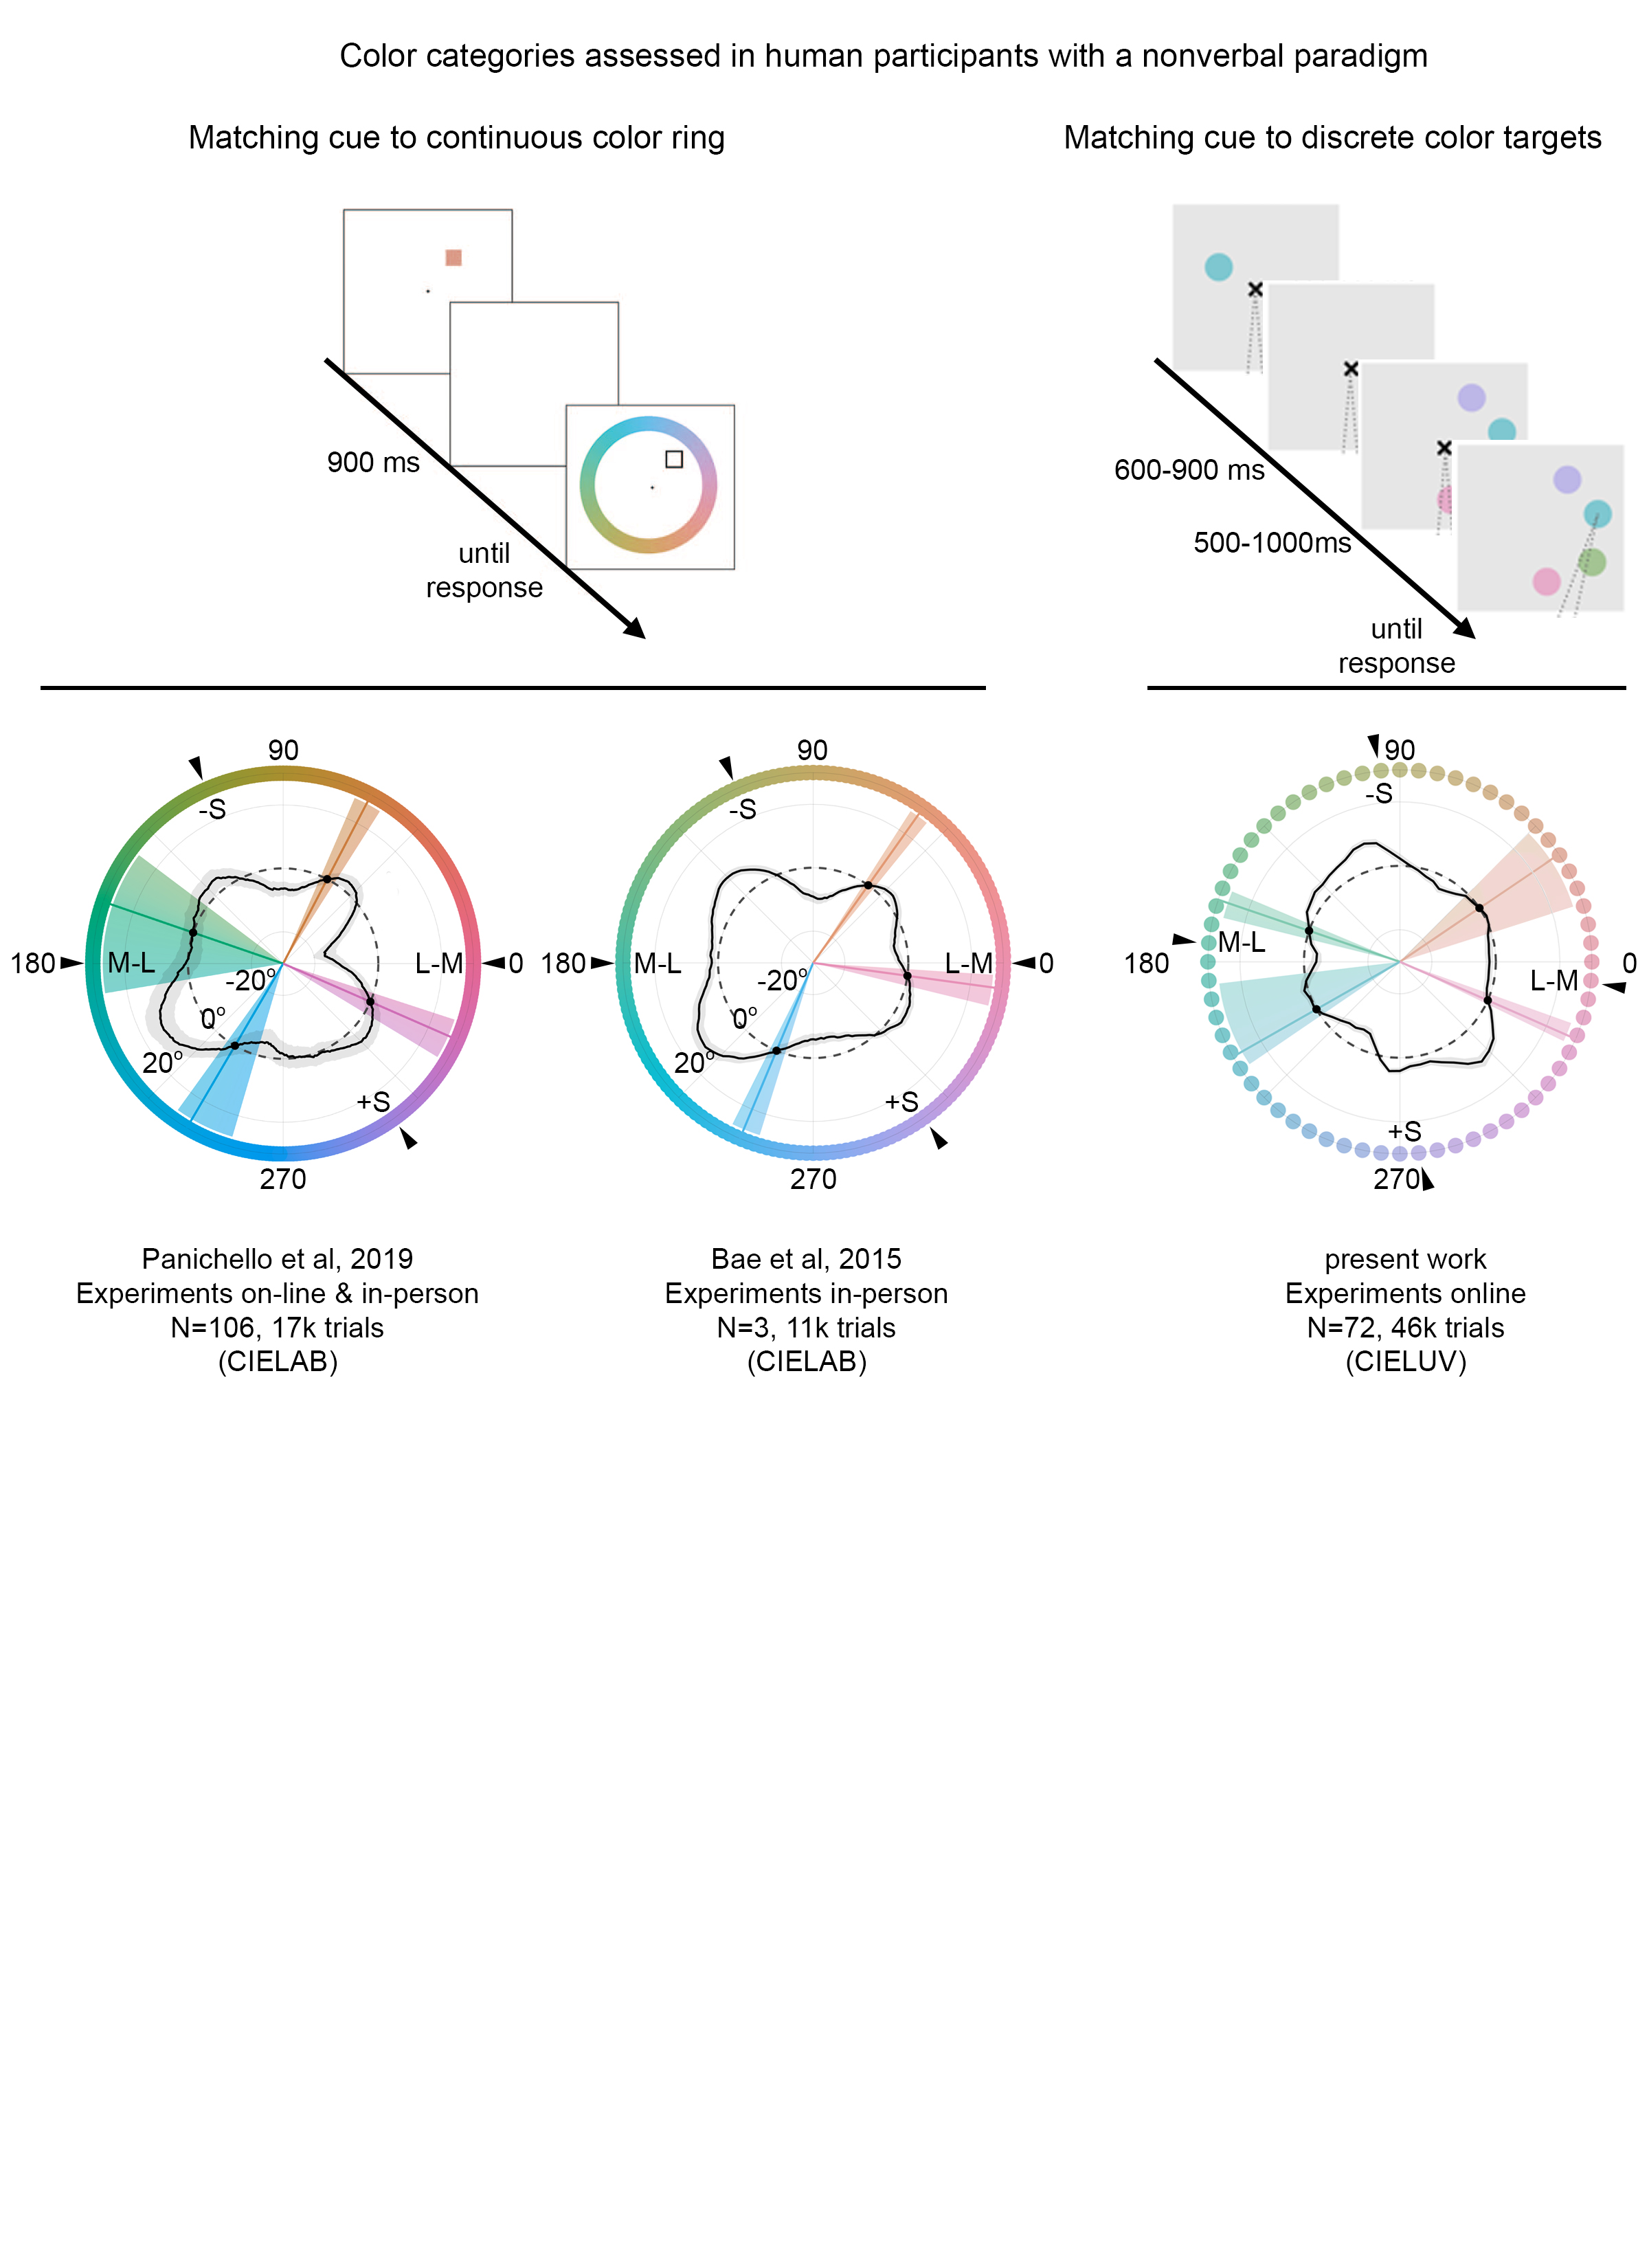
\includegraphics[width=\textwidth+4cm,trim={0 11cm 0 0},clip]{../Figures/flat/SI_Human_2.jpg}
    \caption{\textbf{Color categories assessed in human participants with a nonverbal paradigm. }
    Prior work by \citet{bae_why_2015} and \citet{panichello_error-correcting_2019} has used a task in which participants match the color of a cue to a continuous ring of colors; those published results were obtained with a combination of in-person experiments and on-line experiment, with a memory delay and without. The results are broadly consistent, recovering four color categories by mixture-model analysis, corresponding to blue, green, orange and pink. 
    Note that the data from \citep{bae_why_2015} shown in the figure were from just three participants, engaged in a task that had a memory delay; those authors confirmed the results in more subjects with a version of the task that omitted the memory delay period (the cue and the match-option color wheel were presented simultaneously). The present work adapted the paradigm so that the match options in each trial were four discrete targets randomly drawn from 64 colors sampling the color space. The data shown in this figure were obtained in human participants, with experiments conducted online with Amazon Mechanical Turk. These results are again broadly consistent with the prior work using the continous-matching ring in recovering, by mixture analysis, four significant categories corresponding to blue, green, orange, and pink. We note that the discrete-matching task recovers a trend for a fifth category that would correspond to “purple”; close inspection of the results in \citep{bae_why_2015, panichello_error-correcting_2019} and in studies of human infants \citep{skelton_biological_2017} also show evidence of this trend. The stimuli in the \citep{bae_why_2015, panichello_error-correcting_2019} were defined in CIELAB, while the stimuli in the present work were defined in CIELUV; this difference in color space is associated with a slight clockwise rotation of the cone-opponent axes. The S axis poles provide a useful landmark; they are associated with negative slopes in all three data sets.
    } 
    \label{fig:Human}
    \end{fullwidth}
\end{figure}

\begin{figure}
    \centering
    \begin{fullwidth}
    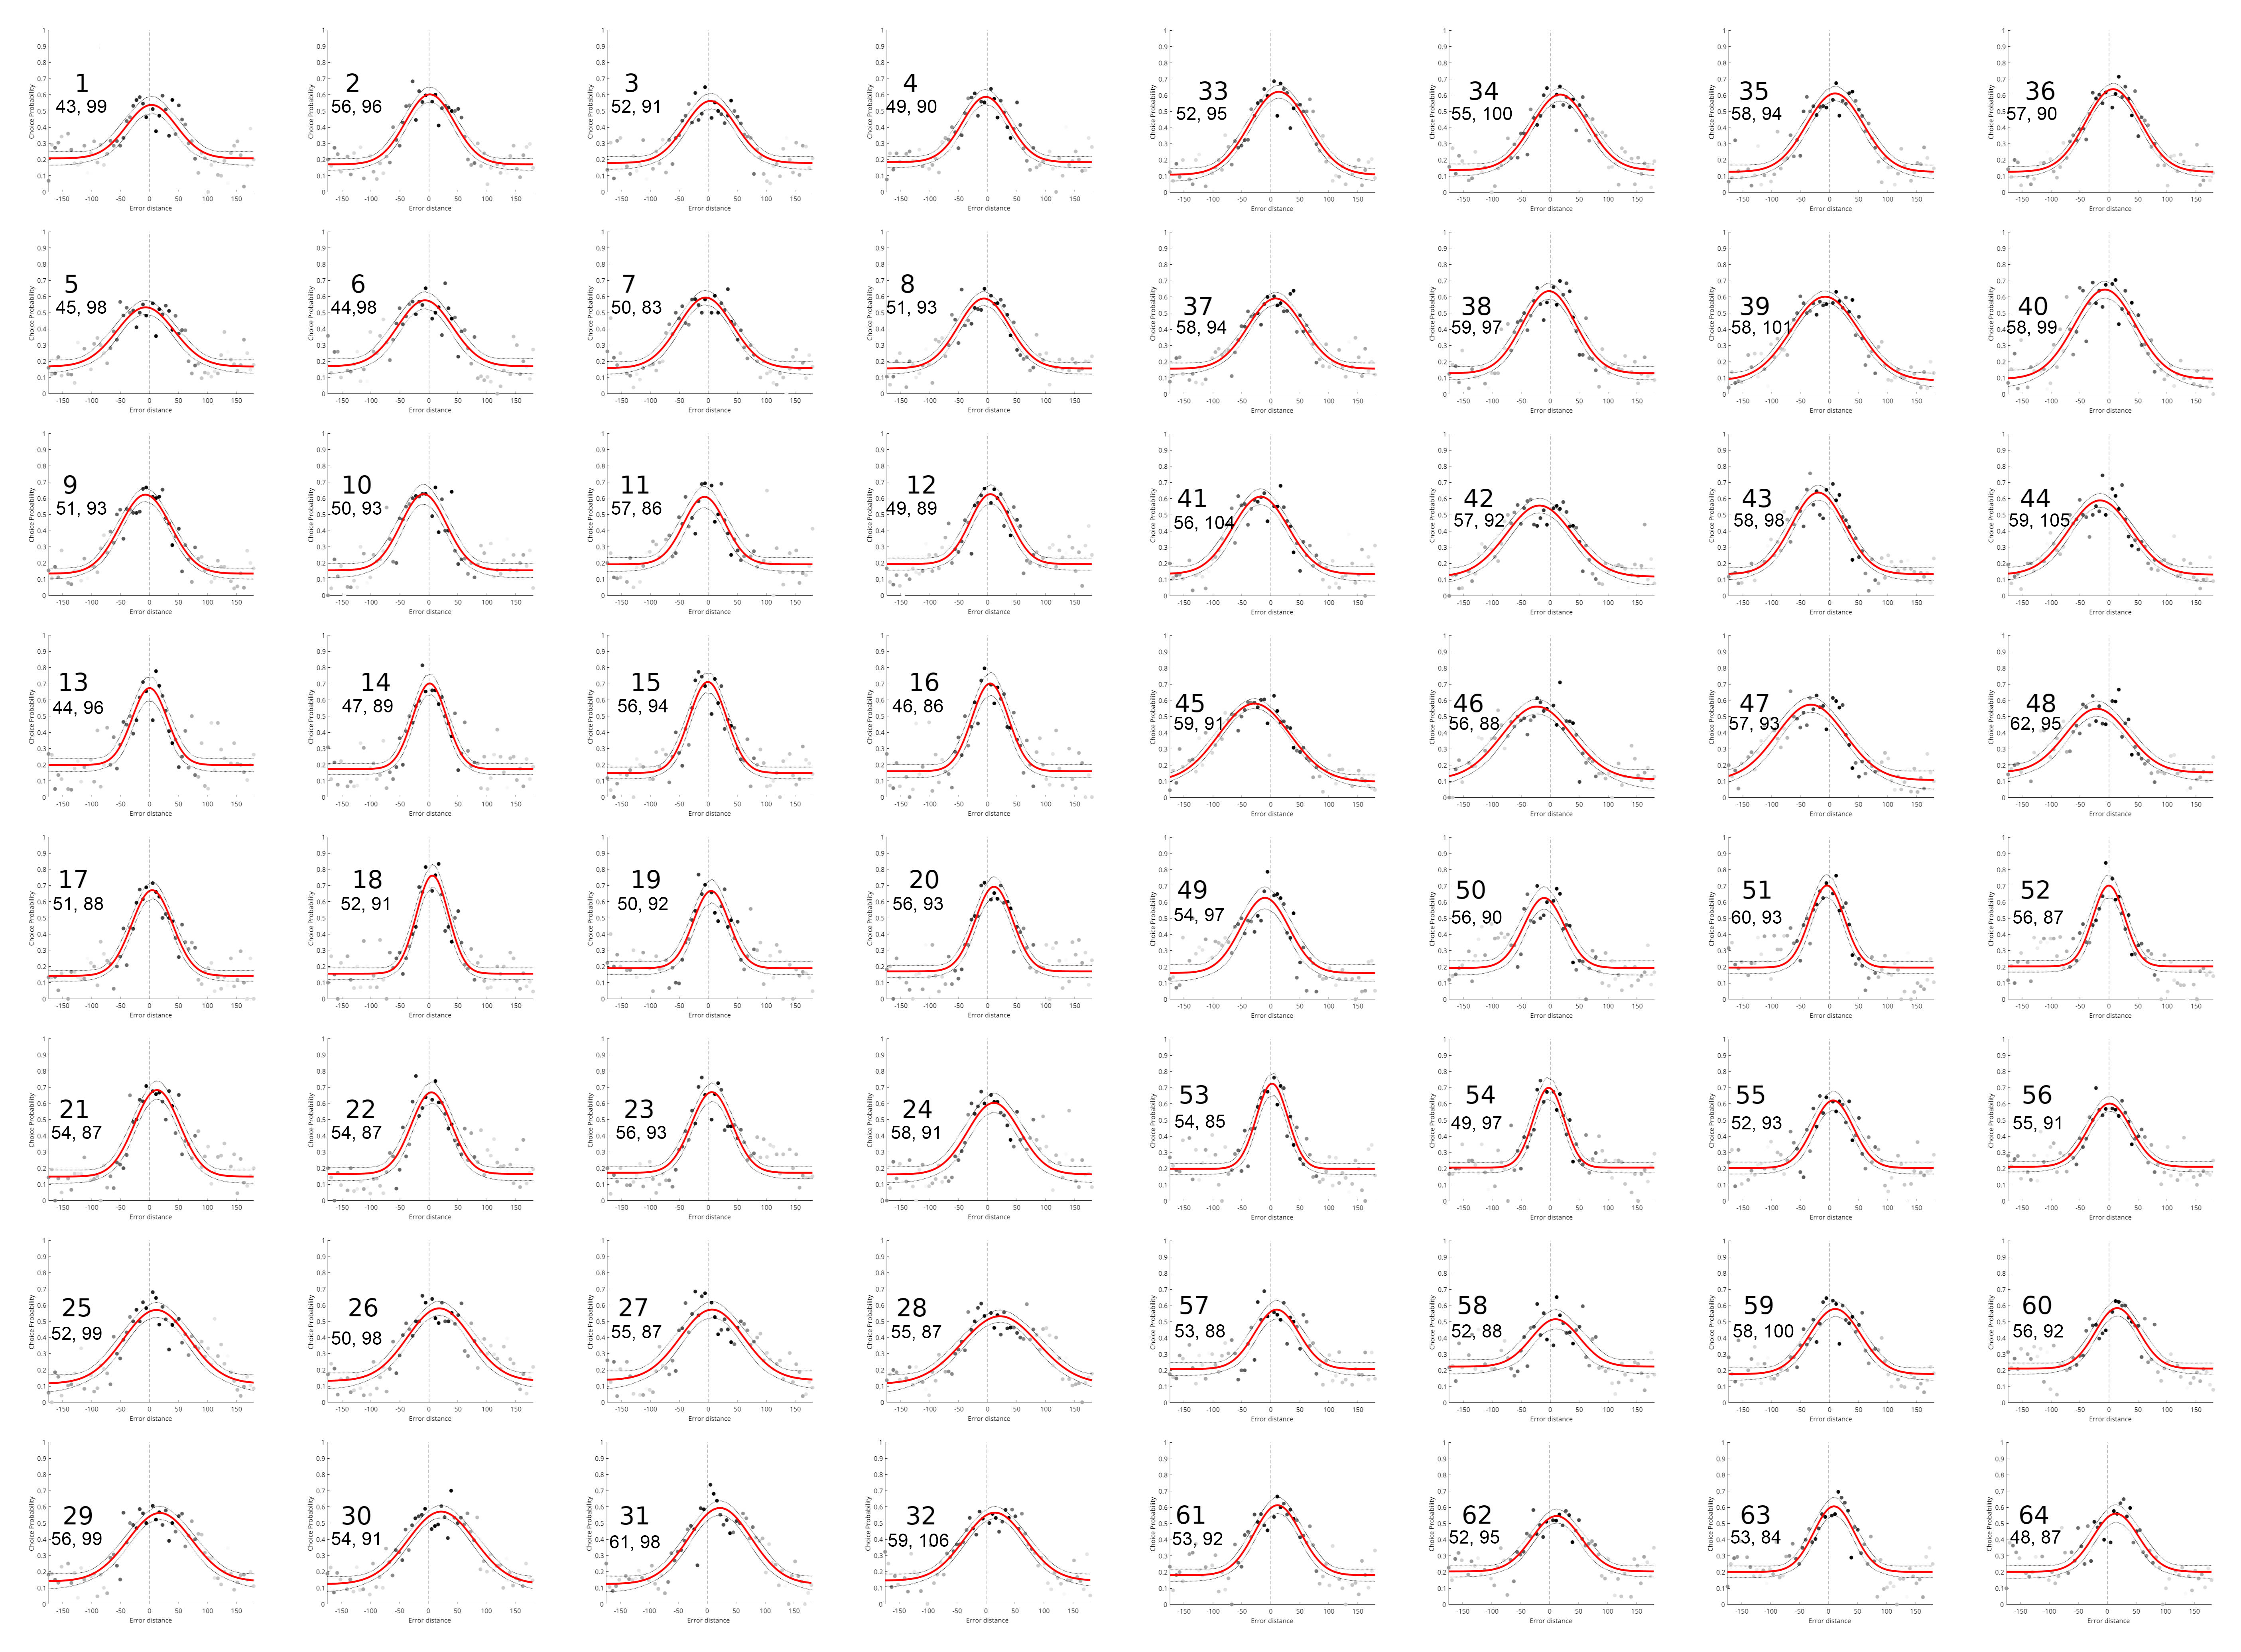
\includegraphics[width=\textwidth+4cm]{../Figures/flat/SI3_MMBreakOut_2.jpg}
    \caption{\textbf{Gaussian fits from the Mixture Model.}
    Each trace shows the Gaussian fit for one of the 64 target colors (large number in each panel corresponds to the cue color) used in the color-matching task, as per Equation 1; data averaged over four animals. The extent to which each data point is black versus white indicates the number of trials that provided that choice option, normalized for each cue (the pair of smaller numbers below the cue-color number provides the range: the larger number corresponds to the black symbol, and the smaller number to white); see Methods for how the curves were fit to the data. 
    } 
    \label{fig:MMBreakOut}
    \end{fullwidth}
\end{figure}

\begin{figure}
    \centering
    \begin{fullwidth}
    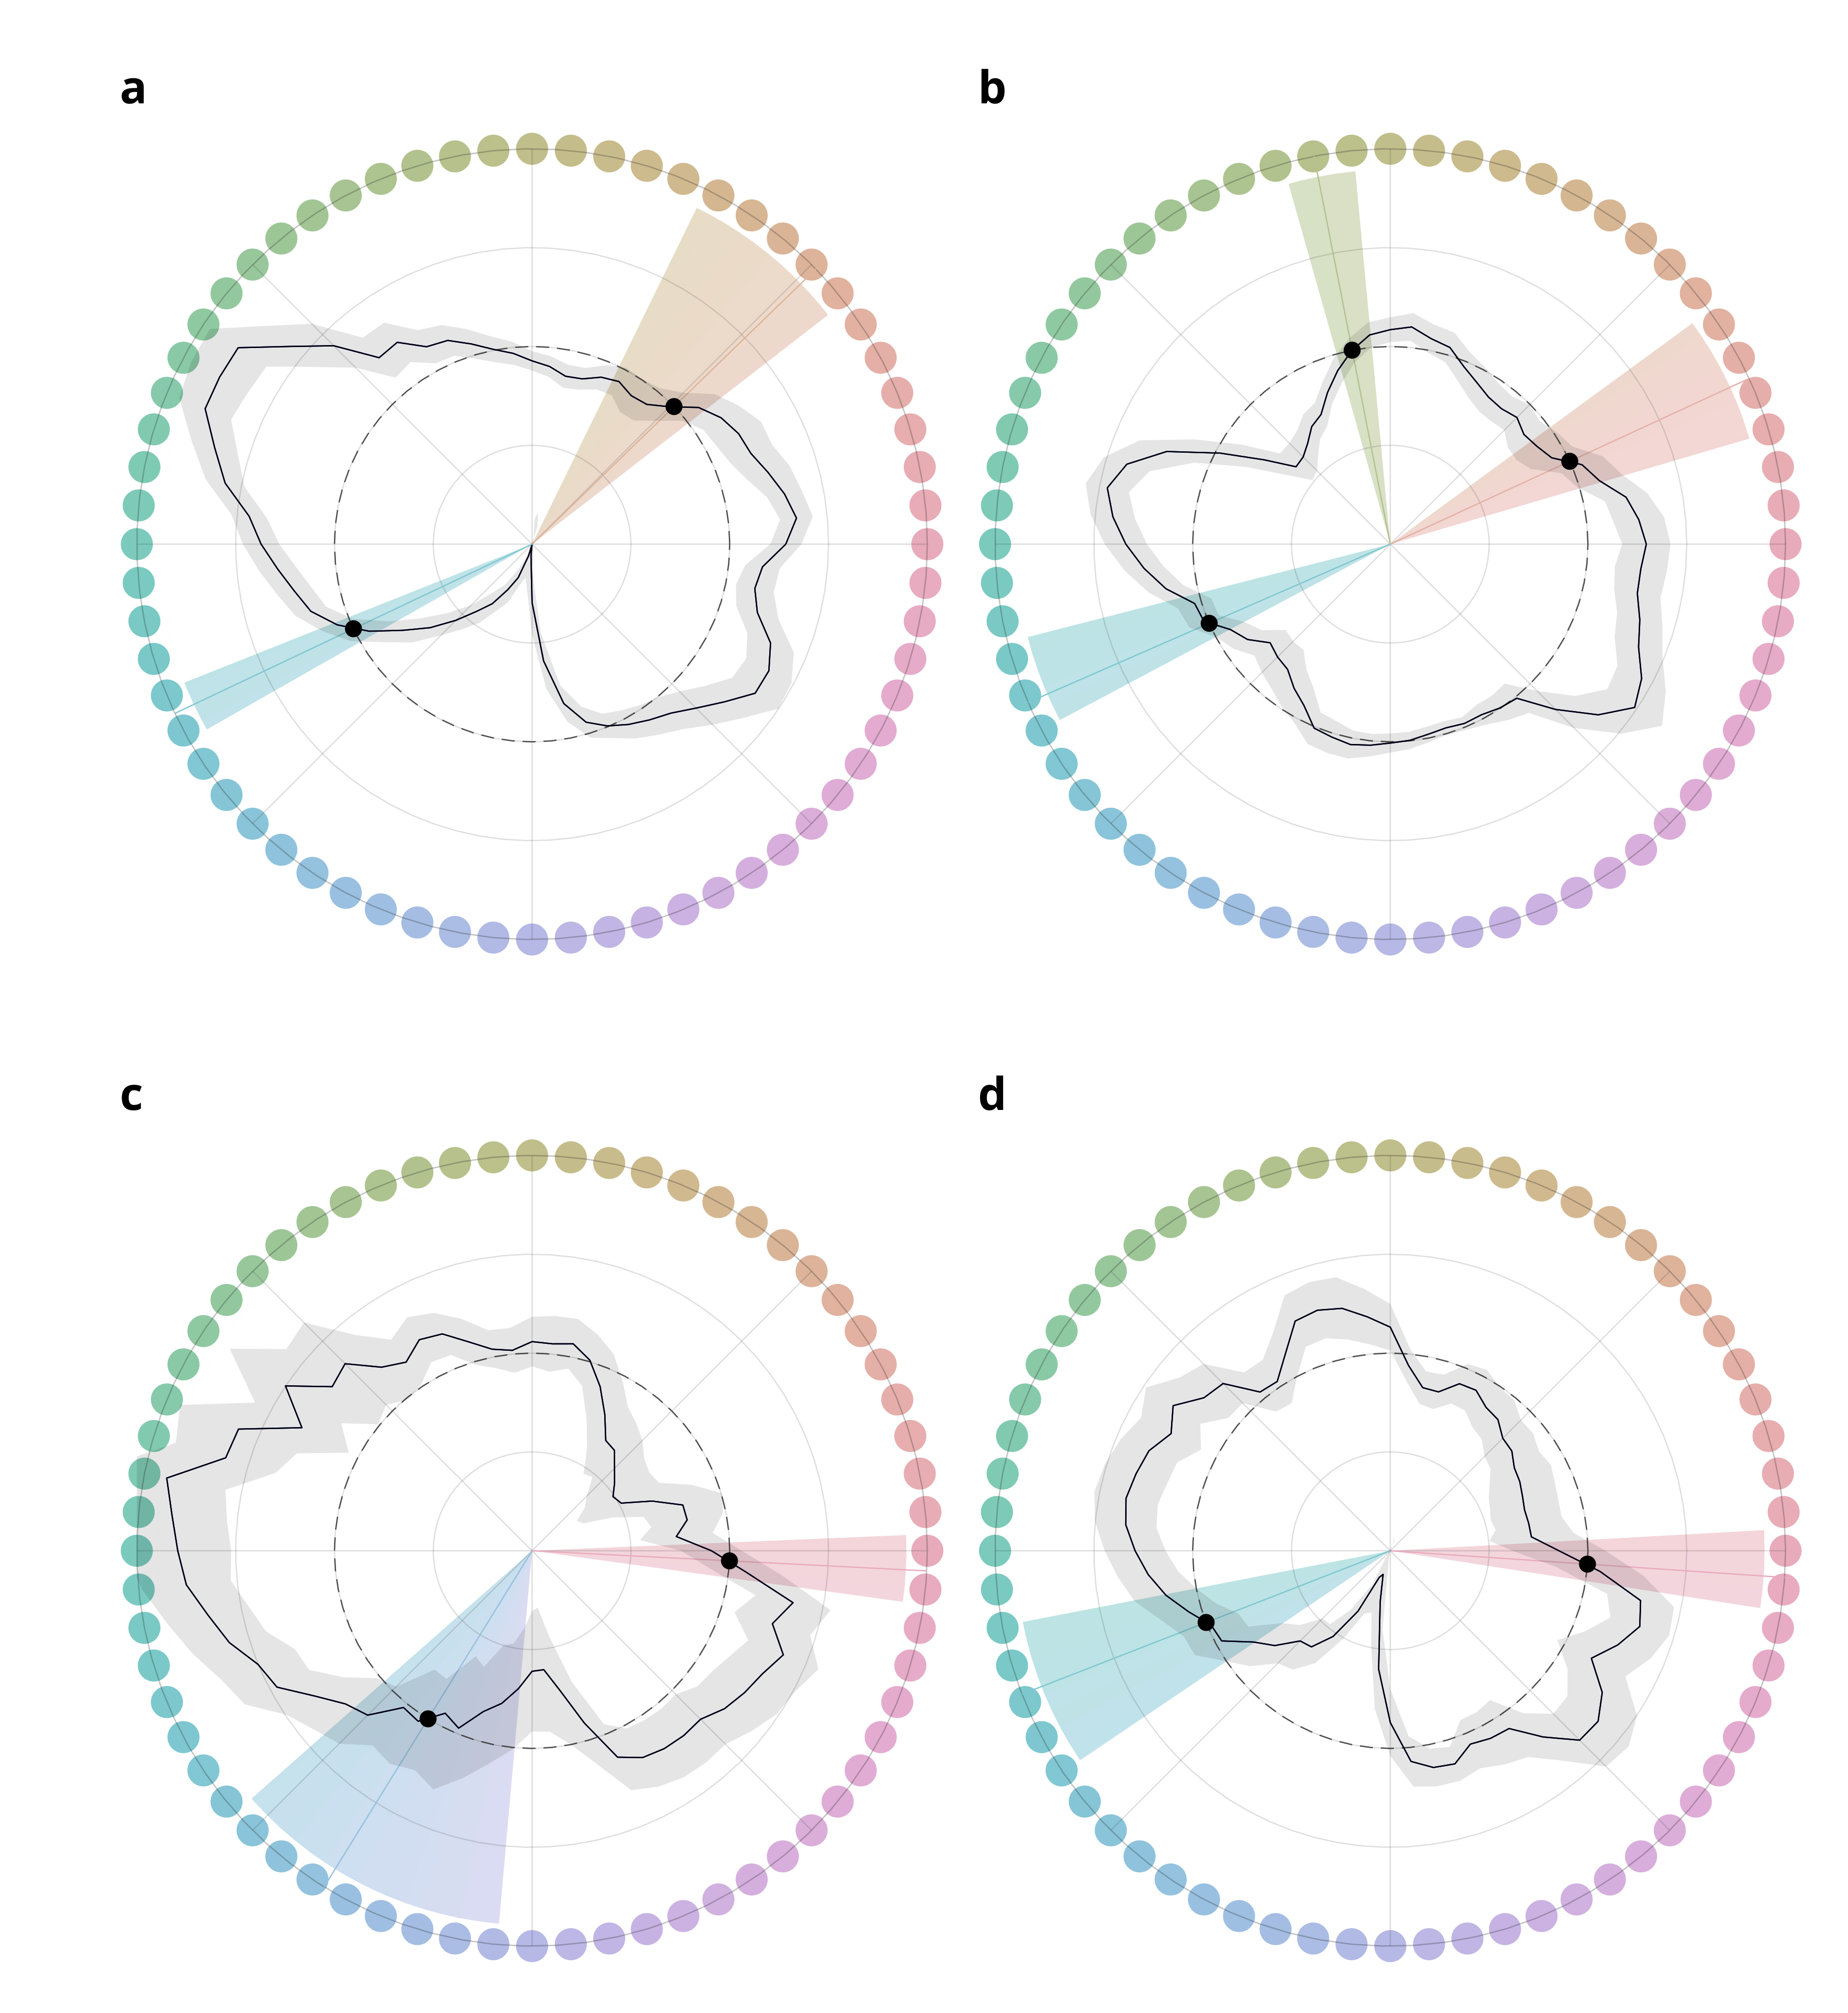
\includegraphics[width=\textwidth+4cm]{../Figures/flat/SI4_MM.jpg}
    \caption{\textbf{Mixture-model analysis of the individual data for the four animals in the color-matching task.}
    Data shown in the same format as Figure 2c; data subsampled to ensure the same amount of data per animal (24526 trials; note that this included all the completed trials for the monkey whose data are shown in panel c).
    } 
    \label{fig:IndiMM}
    \end{fullwidth}
\end{figure}

\begin{figure}
    \centering
    \begin{fullwidth}
    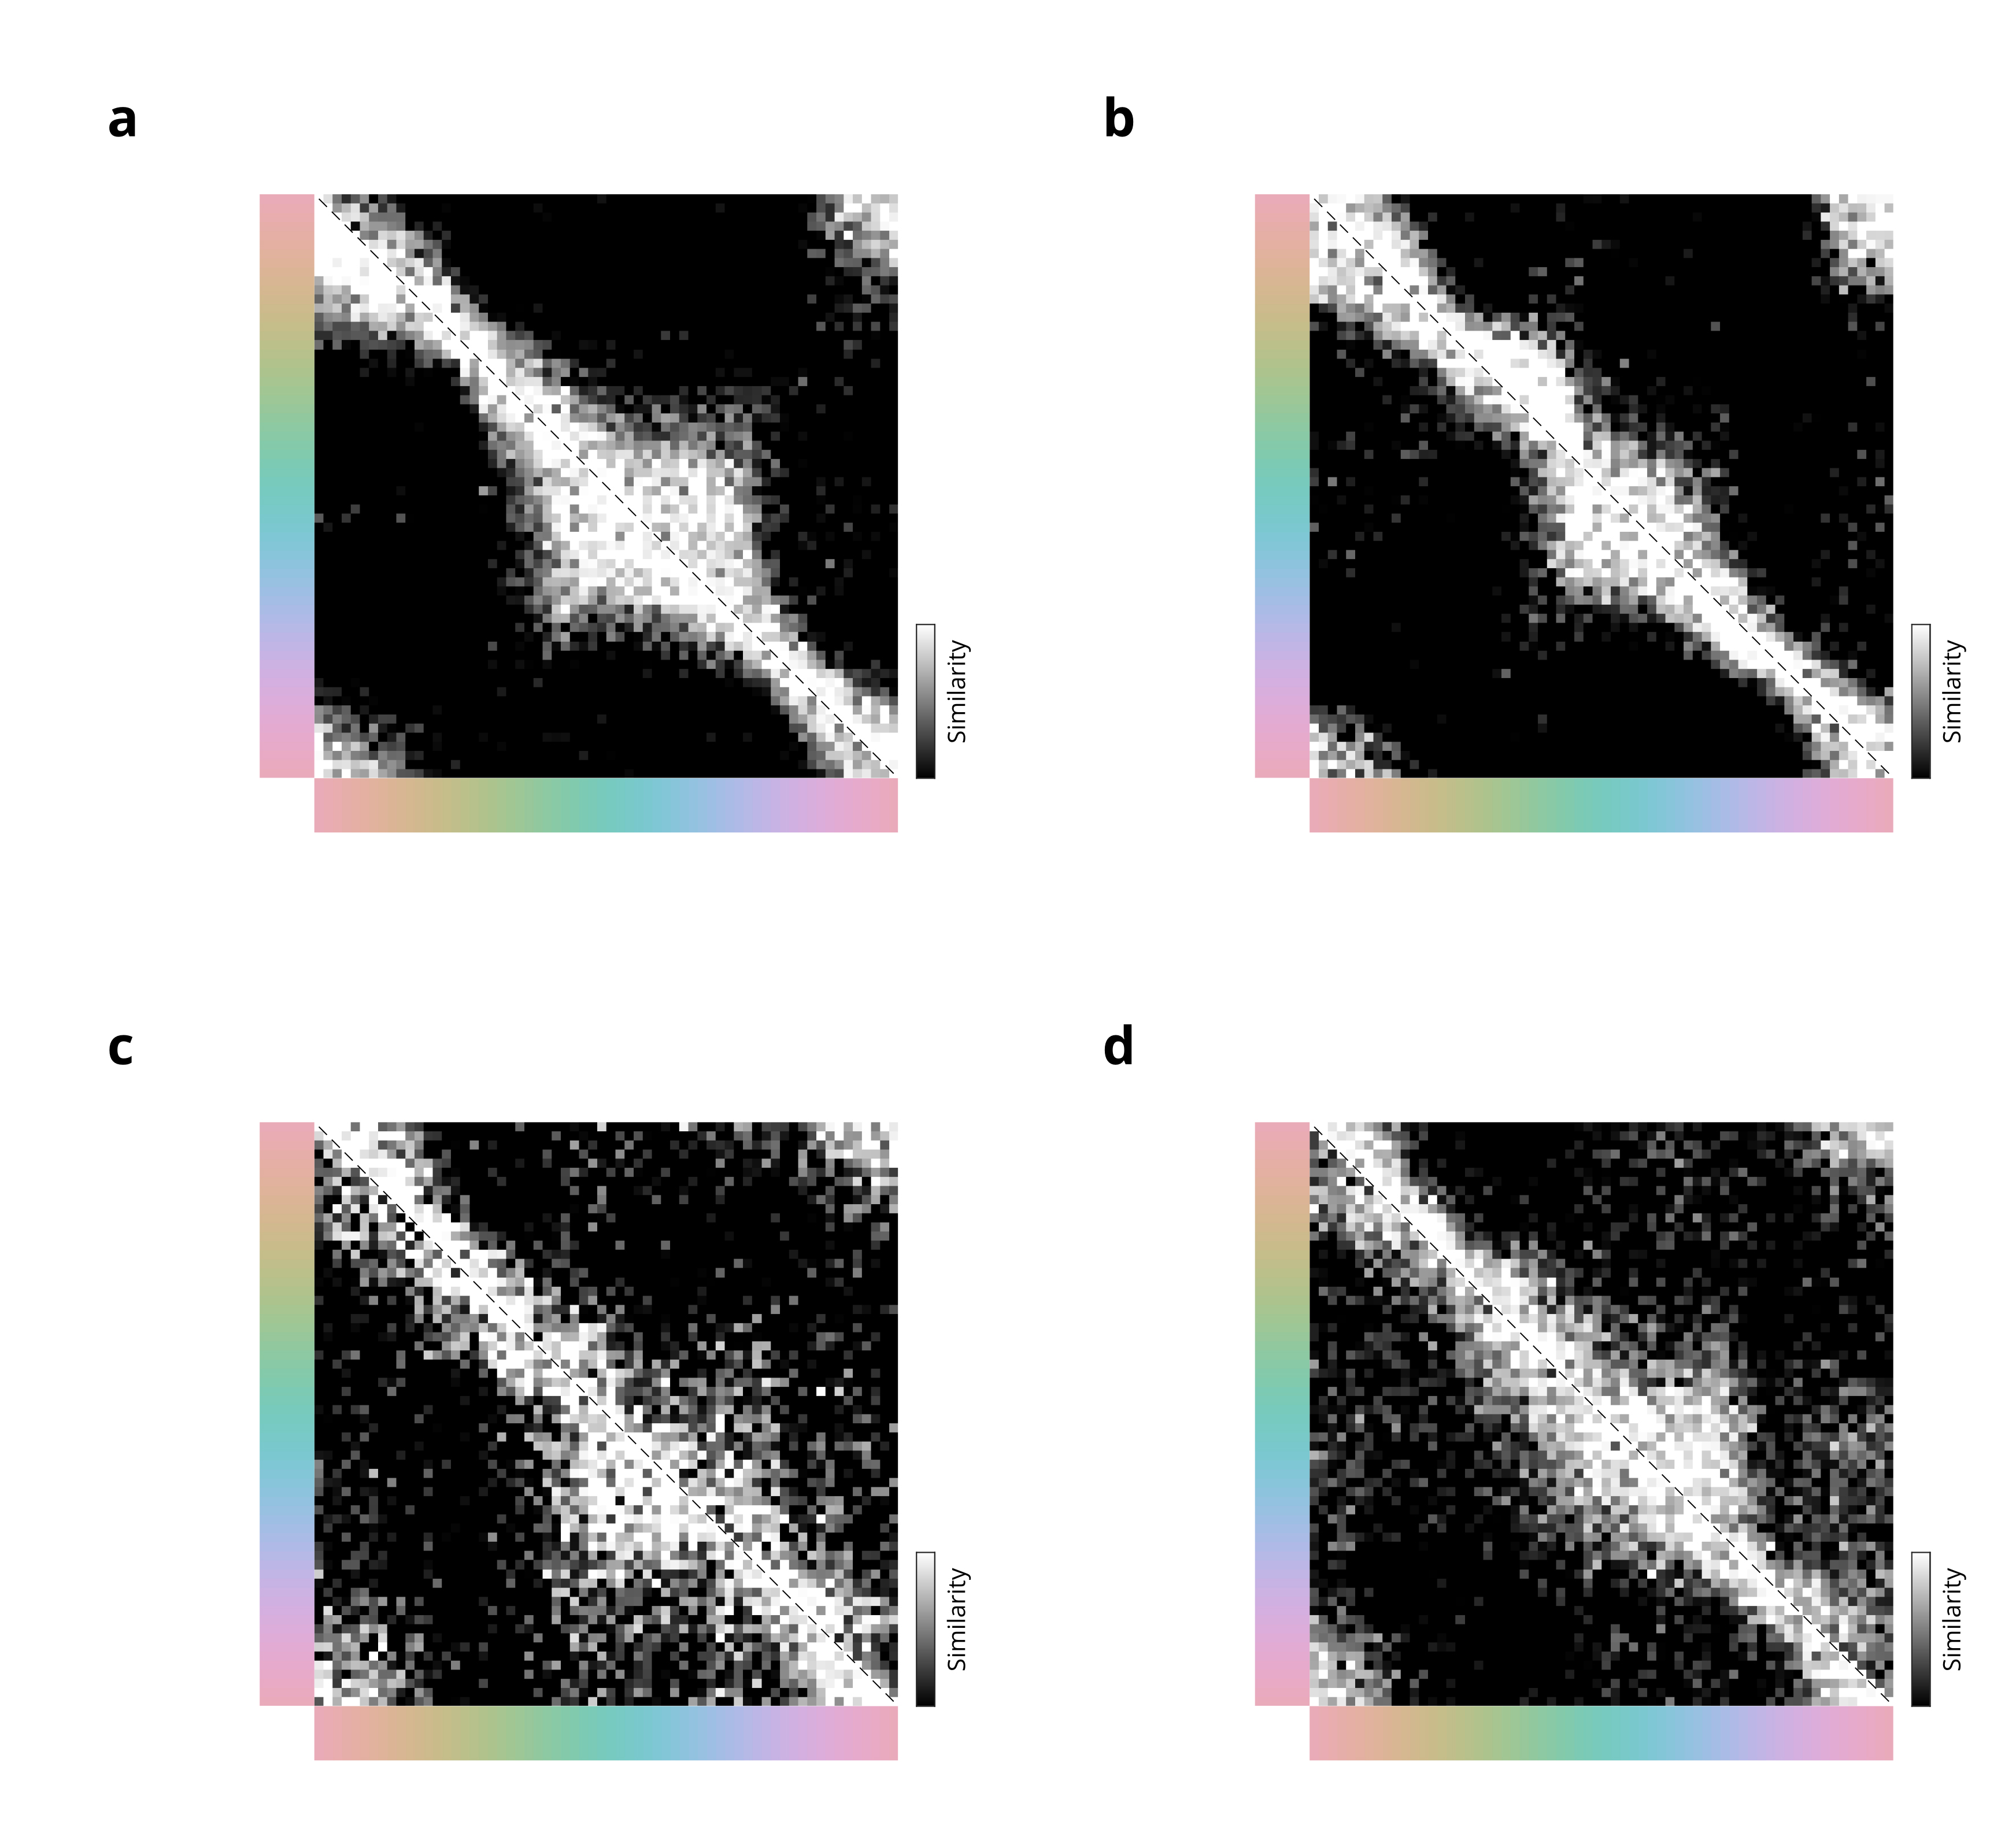
\includegraphics[width=\textwidth+4cm]{../Figures/flat/SI5_IndTCCv.jpg}
    \caption{\textbf{Similarity matrices for free similarity matrix models, fit to individual data.}
    The order of the plots is the same as the order in other figures, PO, CA, BU, MO. See Figure 3ab for data averaged across animals, with data subsamples to ensure the same amount of data per animal.
    } 
    \label{fig:IndiTCC}
    \end{fullwidth}
\end{figure}

\begin{figure}
    \centering
    \begin{fullwidth}
    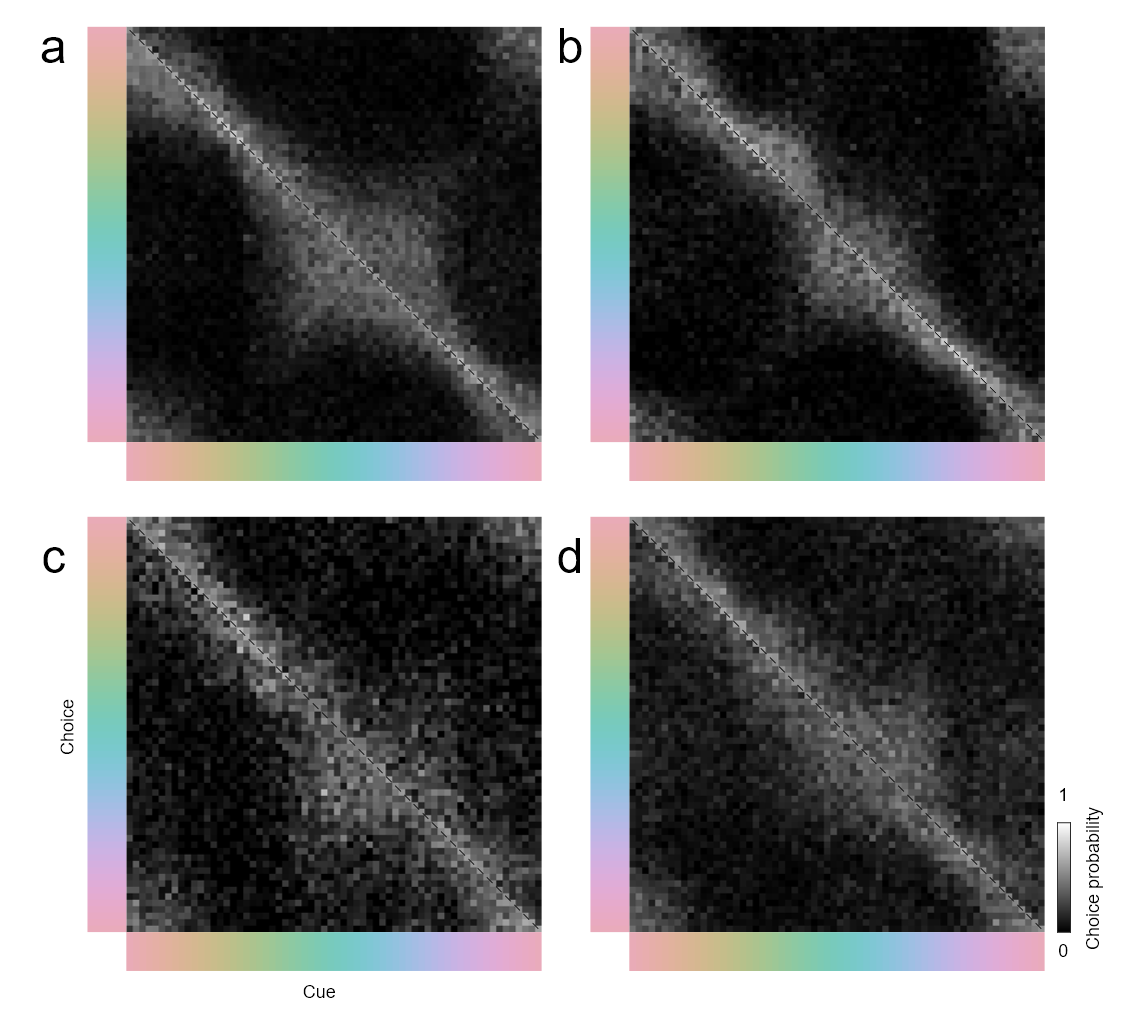
\includegraphics[width=\textwidth+4cm]{../Figures/flat/SI6_choiceMatrices.png}
    \caption{\textbf{Choice probability matrices for free similarity matrix models, for the four individuals.}
    As per the similarity matrices presented, each column represents a cue, and each row represents a choice. 
    Here, however, rather than the similarity between cue/choice pairs we show the probability of selection. 
    Whereas the similarity matrix is the output of model fitting, this matrix is derived more directly from the data: each cell is simply the number of times a particular choice was made divided by the number of times that choice was an option. 
    The identity line, representing correct options, appears artifically inflated (see Methods for further information).
    } 
    \label{fig:choiceProbabilityMatrices}
    \end{fullwidth}
\end{figure}



\clearpage
\printbibliography[title=Methods References]
\end{refsection}


%%%%%%%%%%%%%%%%%%%%%%%%%%%%%%%%%%%%%%%%%%%%%%%%%%%%%%%%%%%%
%%% ARTICLE END
%%%%%%%%%%%%%%%%%%%%%%%%%%%%%%%%%%%%%%%%%%%%%%%%%%%%%%%%%%%%

\end{document}




